\documentclass[times, utf8, zavrsni, numeric]{fer}
\usepackage{booktabs}
\usepackage{listings}
\usepackage{booktabs}
\usepackage{caption}
\usepackage{subcaption}
\usepackage[nobiblatex]{xurl}
\usepackage{setspace}
\usepackage{float}
\usepackage{parallel}
\begin{document}

\tableofcontents

\listoffigures

\listoftables

\chapter{Uvod}
U današnjem digitalnom dobu, arhive predstavljaju izvor neprocjenjivih informacija i povijesnih podataka na kojima se mnoga današnja istraživanja temelje. Međutim, arhive često sadrže i brojne stare dokumente pisane rukom ili pisaćom mašinom i time predstavljaju izazov za efikasnu obradu i pretraživanje. Za rješenje ovog problema primjena metoda optičkog prepoznavanja podataka postaje ključna kako bi se omogućilo digitaliziranje i efikasnije pretraživanje materijala.

Optičko prepoznavanje znakova je metoda koja omogućuje računalima prepoznavanje i interpretaciju prisutnog teksta na slikama ili skeniranim dokumentima. Metode prepoznavanja podataka omogućuju pretvaranje fizičkog teksta u strojno čitljiv tekst i time omogućuje daljnju obradu, analizu i pretraživanje.

Ovaj radi bavi se istraživanjem i primjenom metoda optičkog prepoznavanja podataka nad starom arhivskom dokumentacijom s ciljem digitalizacije, lakšeg pristupa i pretraživanja. Analizirat će se različite metode obrade slike, metode prepoznavanja teksta i njegove interpretacije kao i izazovi i prepreke s kojima se susreće prilikom obrade materijala.
Cilj ovog istraživanja je definirati smjernice i preporuke za primjenu raznih metoda obrade slike i metoda prepoznavanja i interpretiranja, s fokusom na postizanje visoke razine točnosti rezultata.
U poglavljima ovog rada, detaljnije će se istražizi i analizirati metode obrade slike i metode optičkog prepoznavanja znakova.
\pagebreak

\chapter{Opis problema}
Zadatak ovog završnog rada je provesti optičko prepoznavanje znakova nad starom arhivskom dokumentacijom. Skup podataka nad kojim provodimo optičko prepoznavanje čine 3052 slike skeniranih dokumenata pisanih hrvatsko-srpskim jezikom.
\\
\\
Skenirani dokumenti pisani su pisaćom mašinom na papirima različitih dimenzija. Velik broj skeniranih dokumenata nije standardne dimenzije papira, A4 ili A5, i prisutna su fizička oštećenja skeniranih dokumenata, poderan papir i ne cjeloviti dijelovi teksta. Dokumenti su pisani pisaćom mašinom što prouzročuje probleme ne konzinstetnosti razine otiska znakova i razne metode ispravljanja pogrešno otisnutih znakova. U načelu ispravljanje pogrešno otisnutih znakova provedeno je otiskavanjem ispravnog znaka preko pogrešnog, time je postignuto preklapanje dva znaka i smanjenje interpretabilnosti konačnog znaka.
Također zbog neopreznog načina skeniranja velik broj dokumenata skeniran je pod ne konzistentni kutevima, razinama osvjetljenja ili brojem prisutnih dokumenata.
Navedena svojstva predstavljaju problem kod inicijalne obrade slike jer ne predstavljaju ujednačeni skup podataka. Ujednačenost je bitno svojstvo kako bi mogli koristiti iste metode obrade na cijelom skupu podataka i time postigli bolje rezultate u koraku optičkog prepoznavanja. Na slici 2.1. prikazana su navedena svojstva na materijalima.
\\
\\
Nadalje skenirani dokumenti sadržajno se razlikuju. Kroz skup podataka pojavljuju se dokumenti koji sadrže odlomke teksta, tablice brojeva, liste elemenata i razne kratke potvrde. Sadržajna ne konzistentnost predstavlja poteškoće kod definiranja ulaznih podataka sustavu za optičko prepoznavanje, naime definiranjem kako ulazni podatci izgledaju omogućavamo lakše prepoznavanje uzoraka i interpretiranje podatka.

\begin{figure}[H]
        \centering
	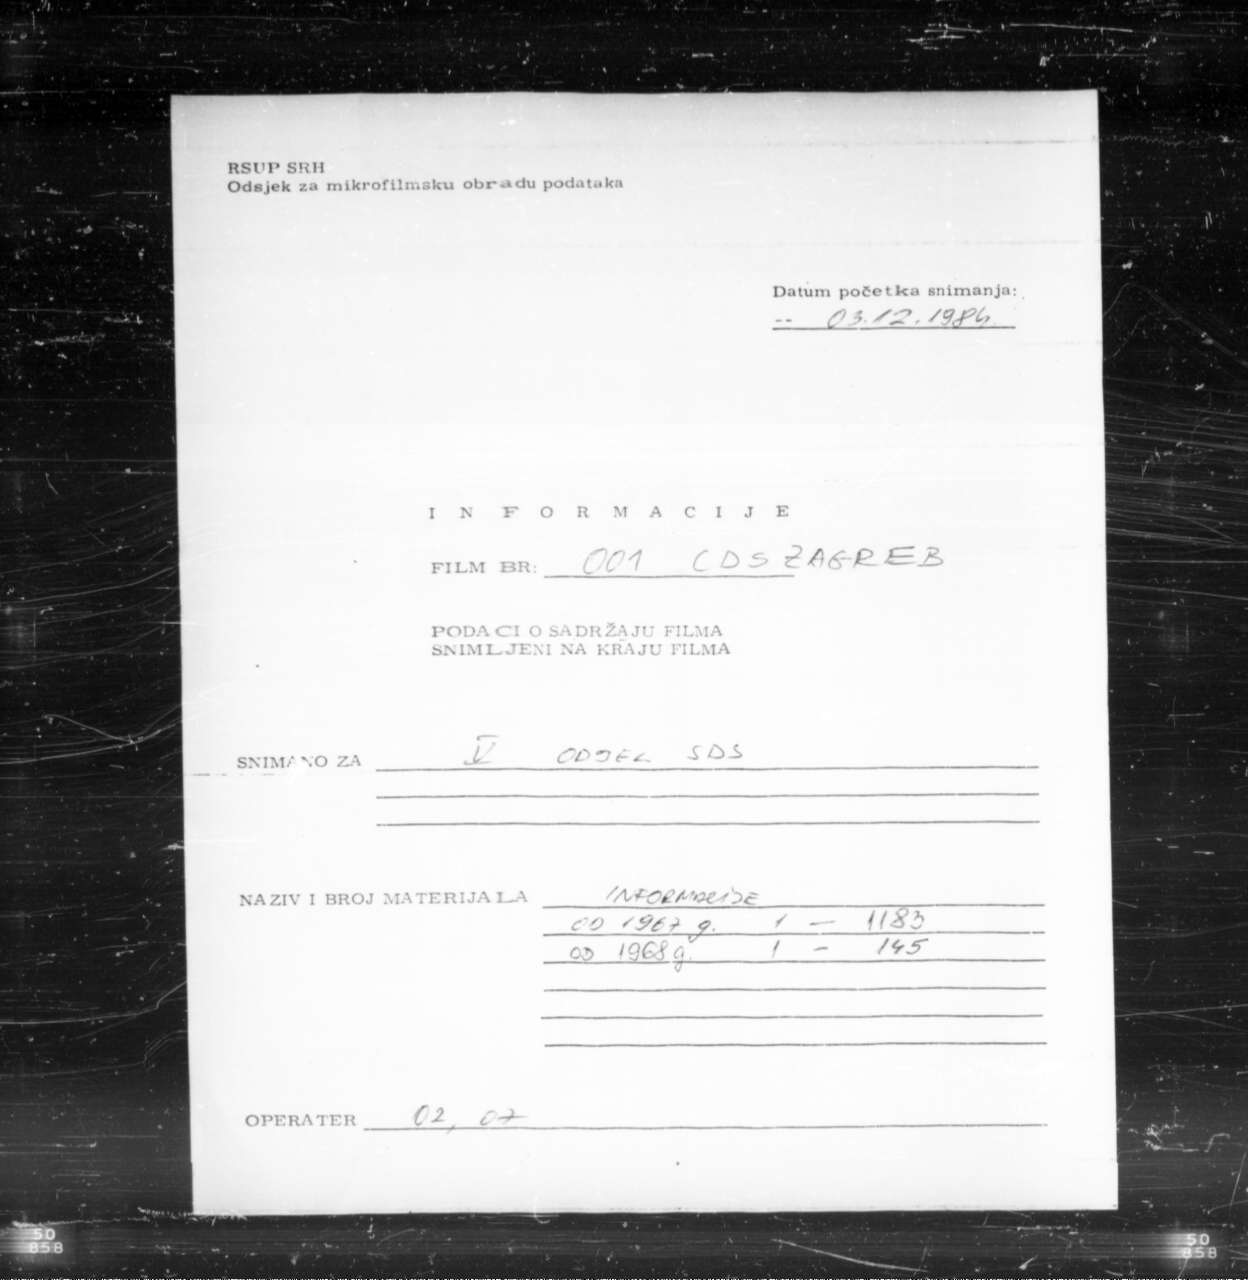
\includegraphics[scale=0.96]{images/opis/Z05353367.jpg}
	\caption{Primjer slike dokumenta sa ručno pisanim tekstom}
	\label{fig:binary_example}
\end{figure}
\begin{figure}[H]
        \centering
	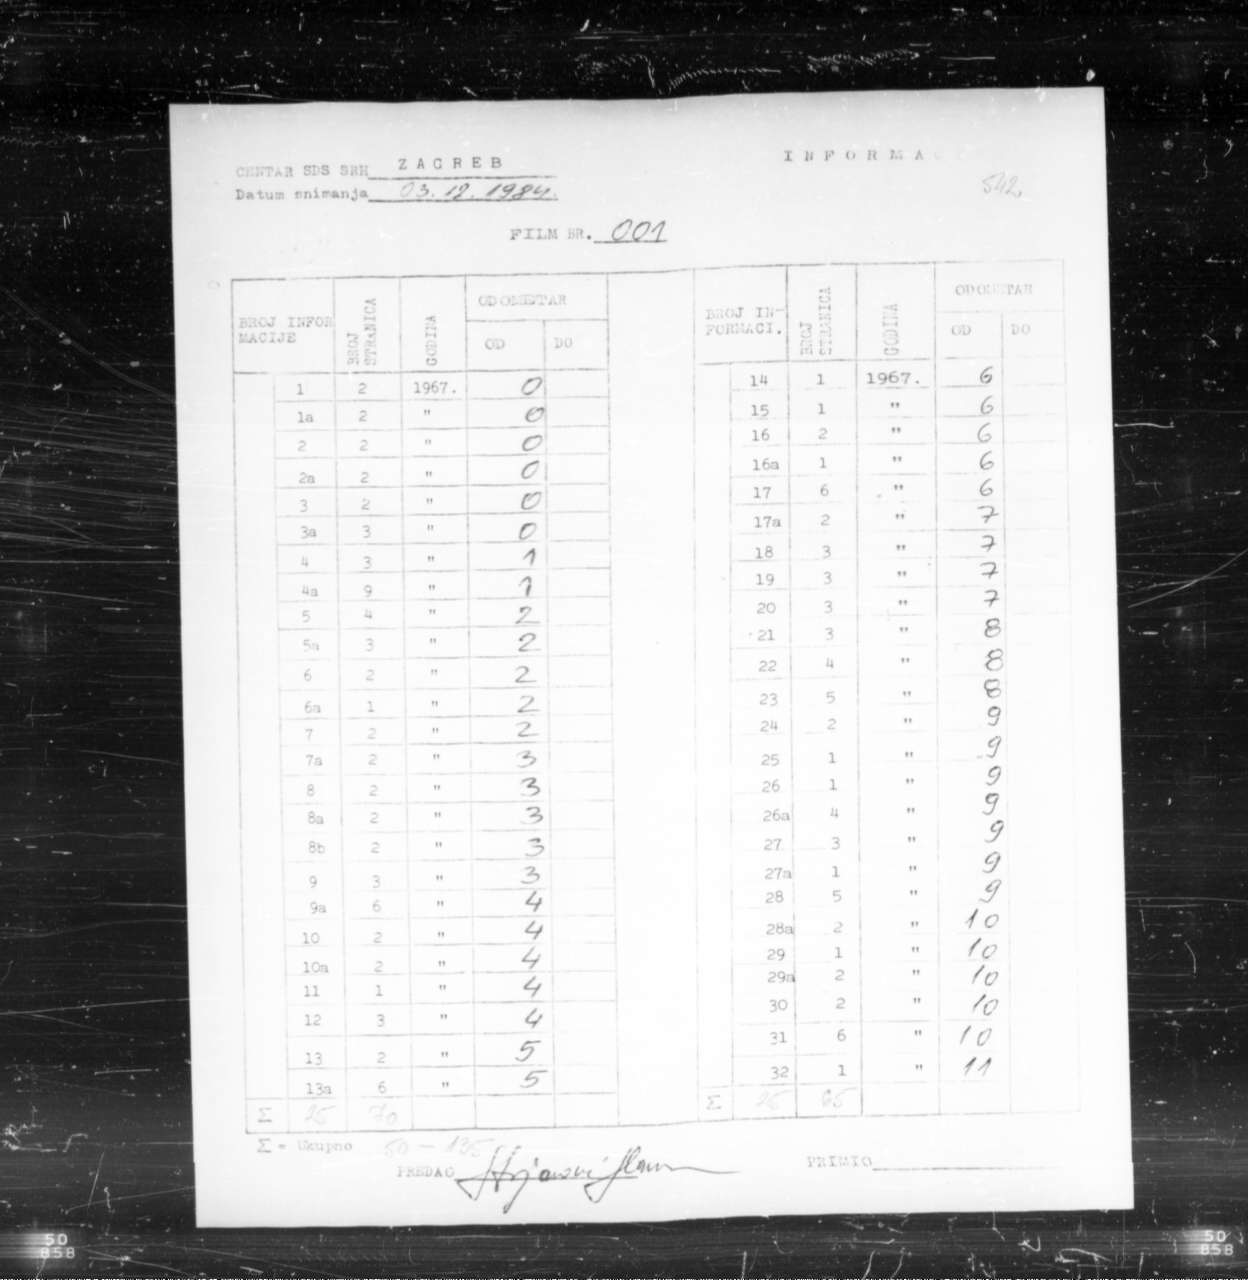
\includegraphics[scale=0.96]{images/opis/Z05353368.jpg}
	\caption{Primjer slike dokumenta sa tabličnim sadržajem}
	\label{fig:binary_example}
\end{figure}
\begin{figure}[H]
        \centering
	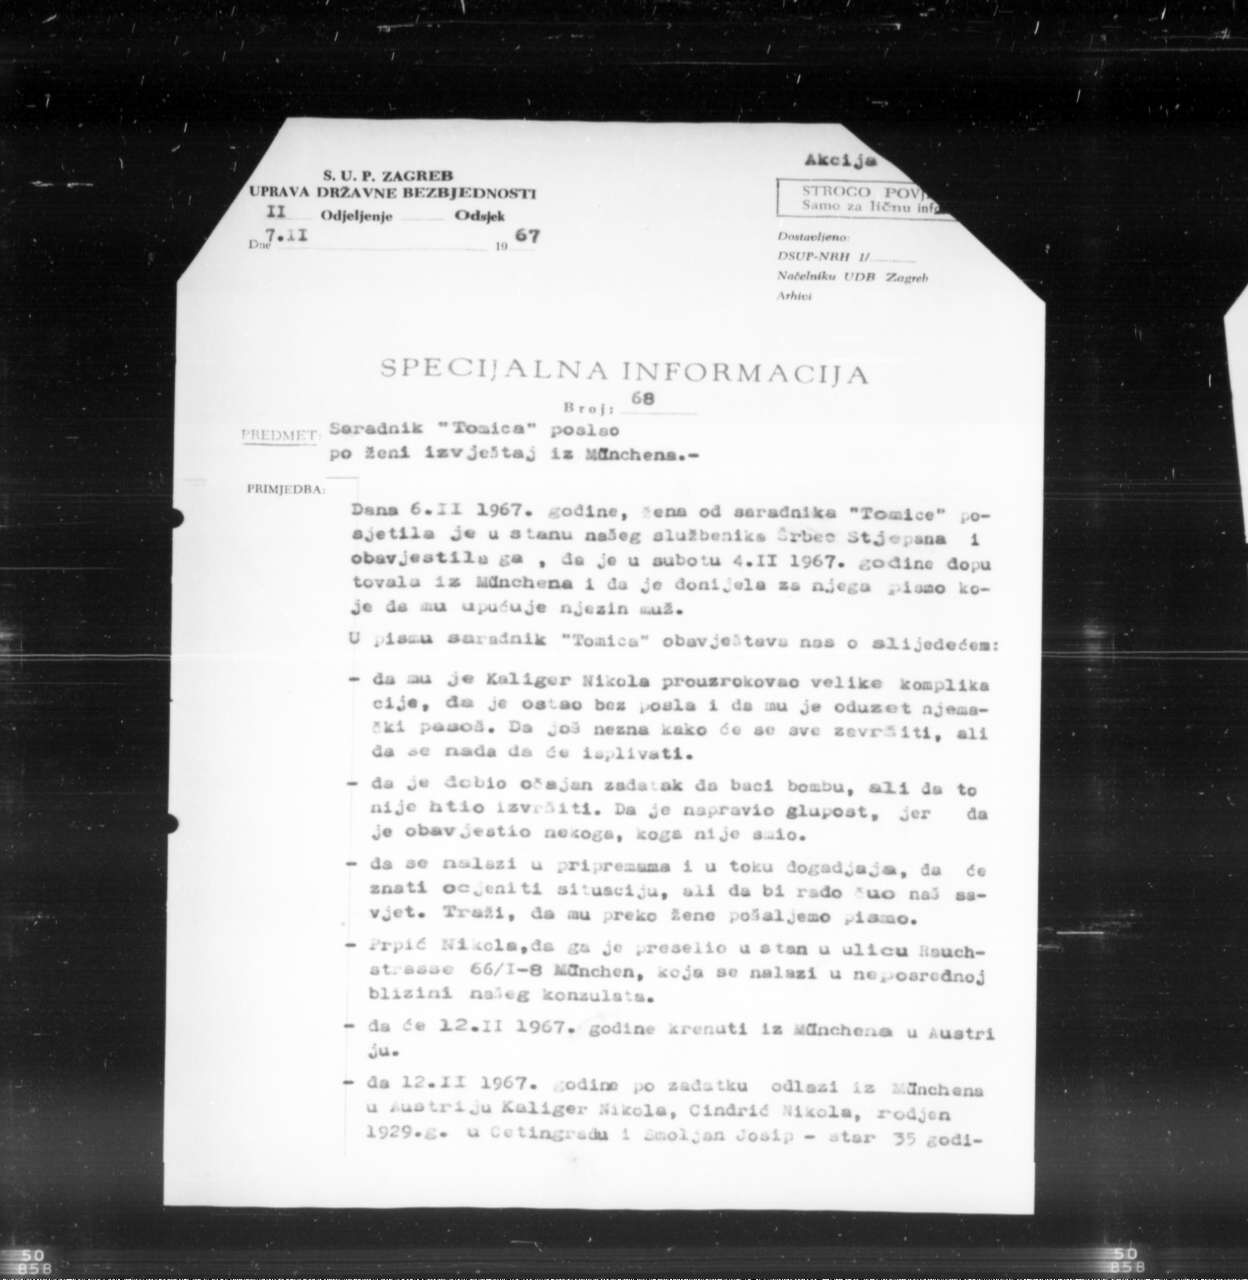
\includegraphics[scale=0.96]{images/opis/Z05353615.jpg}
	\caption{Primjer slike sa dokumentom odlomka teksta}
	\label{fig:binary_example}
\end{figure}
\begin{figure}[H]
        \centering
	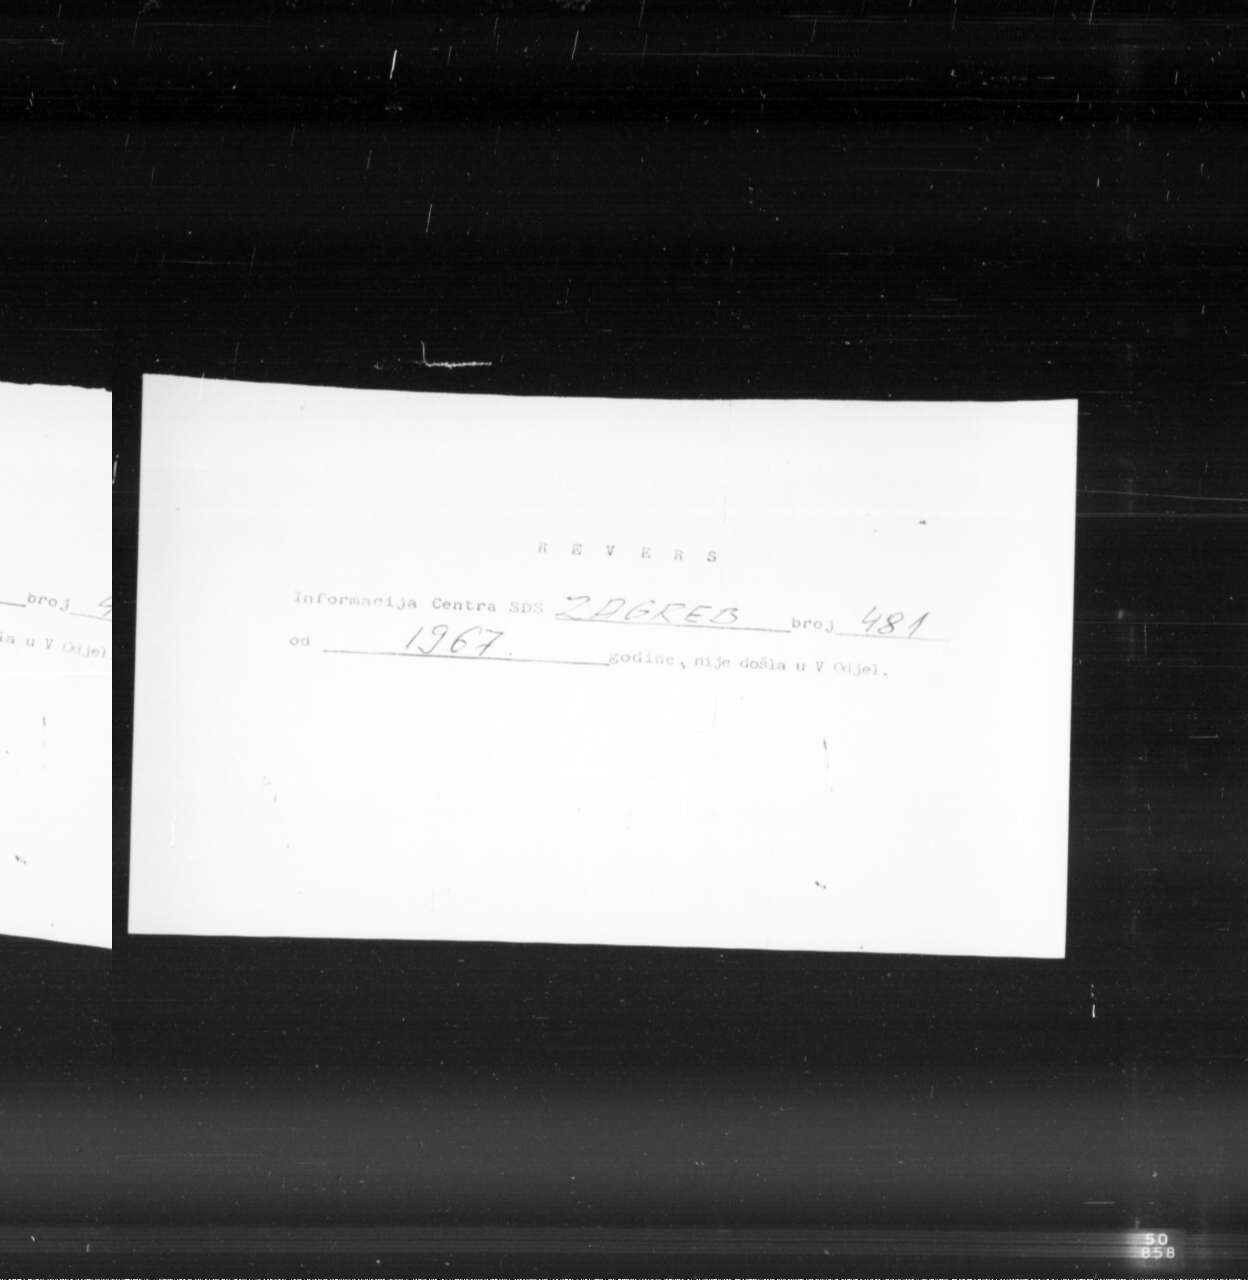
\includegraphics[scale=0.96]{images/opis/Z05354476.jpg}
	\caption{Primjer slike sa dokumentom dimnezije A5, ručno pisanim tekstom i prisutnosti više dokumenata}
	\label{fig:binary_example}
\end{figure}
\begin{figure}[H]
        \centering
	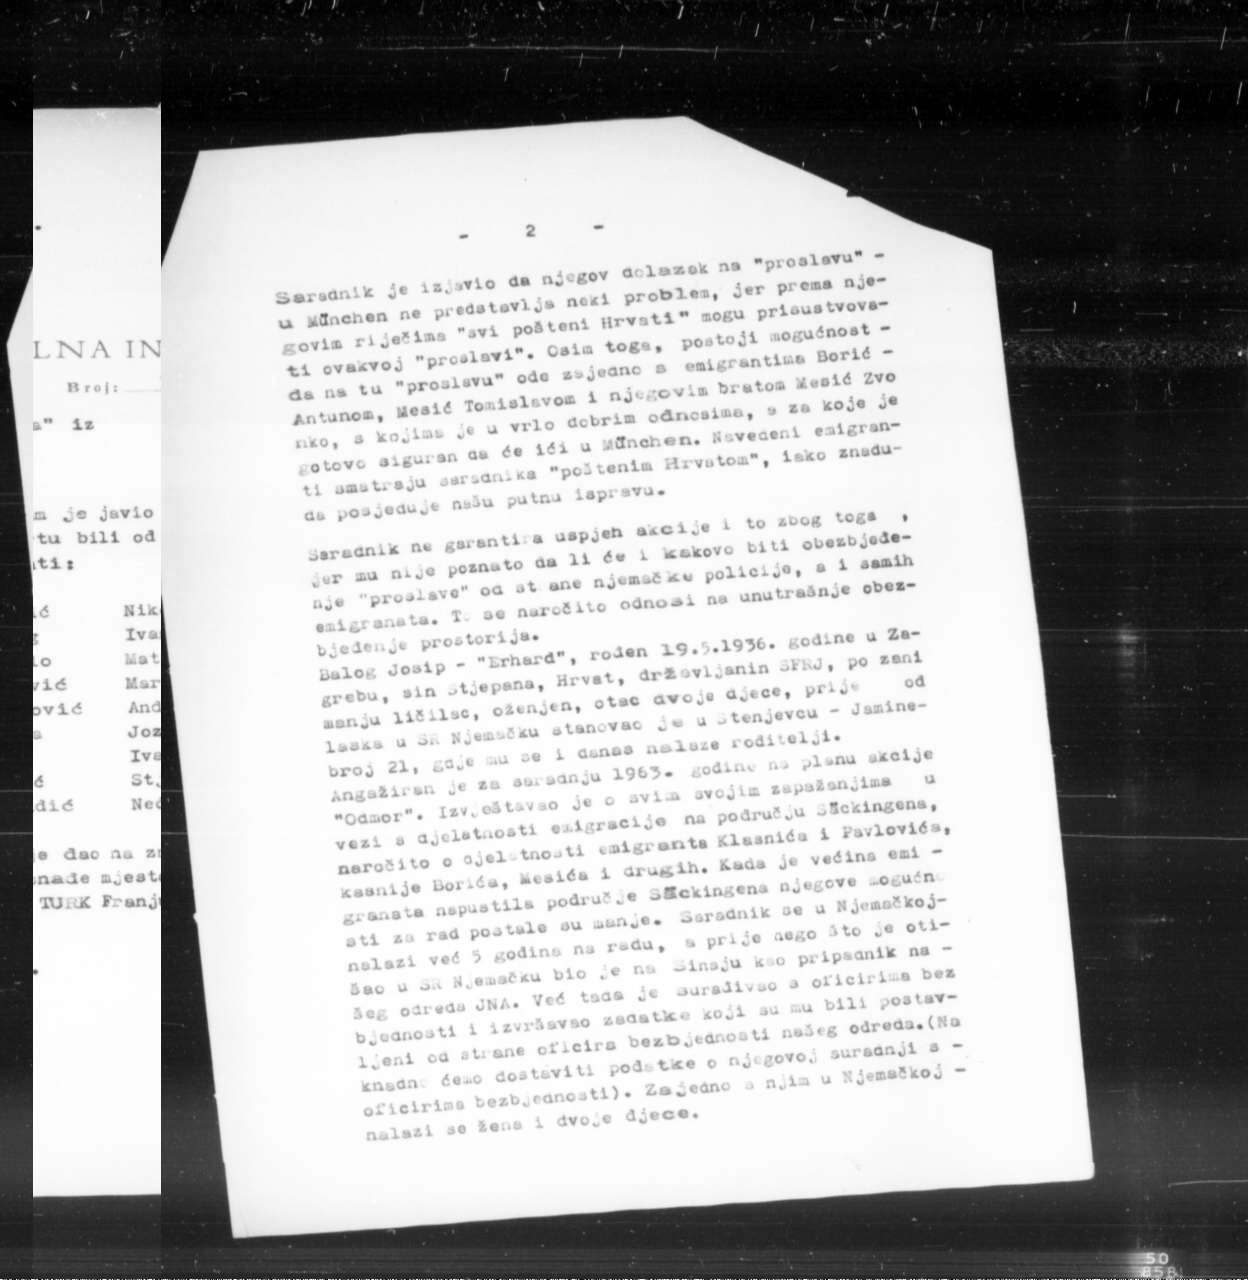
\includegraphics[scale=0.96]{images/opis/Z05353549.jpg}
	\caption{Primjer slike dokumenata sa odlomkom teksta, bez rubova papira, ručno pisanim tekstom i prisutnosti više dokumenata}
	\label{fig:binary_example}
\end{figure}



\pagebreak
\chapter{Korištene tehnologije}
\section{Razvojno okruženje i jezik}
Sustav je razvijen u razvojenom okruženje "Visual Studio Code", još poznat kao "VSCode". VSCode razvila je tvrtka Microsoft za windows, macOS i linux operacijske sustave te je sustav baziran na Electron arhitekturi koja mu omogućava rad na raznim platformama.

Sustav je pisan u programskom jeziku Python odnosno verziji 3.11.1.
Python je programski jezik poznat po svojoj jednostavnoj sintaksi i pristupačnosti početnicima i iskusnim korisnicima. Kreirao ga je Guido van Rossum 1991.godine, u Nizozemskoj. Python karakteriziramo u programske jezike visoke razine zbog jednostavne sintakse i apstrakcije kojom je jednostavan ljudima za čitat i shvatit.


\section{Razvojne biblioteke}
Korištenjem gotovih metode tijekom razvoja sustava iz razvojnih biblioteka OpenCV i NumPy ubrzali smo razvoj, osigurali efikasnost i točnost sustava. 

\subsection{OpenCV}
OpenCV je razvojna biblioteka koju je 1999. godine razvila tvrtka Intel u programskom jeziku C++. Iako napisana u C++, OpenCV biblioteka sadrži podršku za Python i Java programske jezike. U razvoju sustava koristili smo OpenCV verziju 4.7.0.68. i opencv-contrib-python 4.7.0.72.

OpenCV pruža širok spektar metoda i alata iz područja obrade slike i računalnog vida. Glavne funkcionalnosti koje omogućuje OpenCV su: osnovne i napredne metode obrade slike, detekcija i praćenje objekata i računalni vid. OpenCV biblioteka ima široku upotrebu u raznim sustavima koji zahtijevaju obradu, neki do njih su: robotika, sigurnost, medicinska dijagnostika, računalni vid, virtualna stvarnost i prepoznavanje uzoraka. Zbog svoje jednostavnosti, široke podrške i funkcionalnosti izuzetno je popularna među istraživačima, inženjerima i programerima.

\subsection{Numerical Python}
Numerical Python ili poznatija kao NumPy, je razvojna biblioteka za programski jezik Python. Razvio ju je Travis Oliphant 1995. godine u programskim jezicima Python i C.
NumPy nudi efikasne metode obrade polja, matematičkih izračuna i alate za numeričke izračune. Polja primjena NumPy biblioteke su: linearna algebra, statistička analiza podataka, manipulacija poljima i strojno učenje.


\section{Super Resolution}
Super Resolution \cite{superRes} je proces poboljšanja rezolucije i kvalitete slike ili videa korištenjem naprednih algoritama i tehnika. Cilj Super Resolution procesa je postići sliku ili video visoke rezolucije i kvalitete od početne slike ili videa niske rezolucije. Primjenu pronalazimo u poljima računalnog vida, pretprocesiranja slika i video nadzora, gdje slike visoke rezolucije su poželjne za bolje rezultate analize i obrade slike ili videa.
\\
\\
Neki od pristupa kojim možemo postići željeni cilj:
\begin{itemize}
  \item Single-image super resolution 
  \item Multi-image super resolution
  \item Deep learning-based super resolution
  \item Real-time super resolution
\end{itemize}
\hfill \break
Za potrebe ovog rada koristit ćemo "Single-image super resolution". U ovom pristupu poboljšavamo rezoluciju jedne slike niske rezolucije primjenom metoda interpolacije i dubokih neuronskih mreža.
\pagebreak

\section{Tesseract OCR}
Tesseract OCR \cite{tesseract} je sustav za optičko prepoznavanje znakova. Razvila ga je tvrtka Hawlett Packard 1980-ih za internu upotrebu te je objavljen 2005. godine kao open-source projekt. Od 2006. godine njegov razvoj podupire Google. 

Glavna upotreba Tesseract-a je prepoznavanje tiskanog teksta na raznim jezicima. Korištenjem metoda strojnog učenja, posebno neuronskih mreža, analizira i klasificira pročitane znakove. Unutar dijela teksta znakove prepoznaje korištenjem metoda pretprocesiranja slika, izvodi tekstualne znakove i prepoznavanjem uzoraka ih klasificira u već poznate znakove.
\hfill \break
\hfill \break
Neke od značajki Tesseract sustava:
\begin{itemize}
  \item Podrška raznih jezika
  \item Visoka točnost 
  \item Mogućnost pretprocesiranja slika
  \item Treniranje sustava na vlastitim podatcima
\end{itemize}
\hfill \break
Danas uporabu Tesseract sustava nalazimo u automatizirani sustavima za unos podataka, prepoznavanje teksta na slici i upravljanja bazom dokumenata. Za potrebe ovog rada sustav Tesseract koristimo za isčitavanje teksta sa stare arhivske dokumentacije pisane pisaćom mašinom.
\pagebreak

\chapter{Opis rada sustava}
U sljedećim potpoglavljima detaljno ćemo opisati rad sustava za pretprocesiranje slika, objasniti njegovu ulogu za krajnji rezultat i rad sustava optičkog prepoznavanja znakove i načina njegove primjene nad pretprocesiranim slikama\cite{nanonets}, \cite{guideOCR}.

\section{Pretprocesiranje slika}
Prije predaje slika sustavu za optičko prepoznavanje znakova slike prolaze proces pretprocesiranja. Općenito pretprocesiranje podataka uključuje pripremu i obradu podataka kako bi eliminirali dijelove  koji nam nisu potrebni u sljedećem procesu. Za potrebe ovog rada u proces pretprocesiranja uključujemo razne metode obrade slika, skripte za računanje i detekciju raznih značajki prisutnih na slikama te predtrenirani model za poboljšanje rezolucije i kvalitete slike. Svakim korakom pretprocesiranja eliminiramo dio slike koji ne predstavlja značaj u sljedećem koraku ili dio kojim bi sljedeći korak radio otežano odnosno krivo.

\subsection{Početni skup podatka}
Skup podataka nad kojim provodimo pretprocesiranje sadrži 3052 slike. Svaka slika predstavlja skeniranu stranicu stare arhivske kolekcije pisane pisaćom mašinom. Skenirani dokumenti pojavljuju se u raznim dimenzijama, rotacijama, vrsta sadržaja kojeg prikazuju, i kuta skeniranja. Prvim pogledom na skup podataka koji nam je dostupan možemo uočiti da nećemo koristiti globalne postavke obrade za sve slike zbog razlika koja svaka slika sadrži s obzirom na ostale. Zbog toga koristimo razne funkcije kojima određujemo parametre kojima postižemo najbolje rezultate za svaku sliku pojedinačno.
\\
Iz originalnog skupa podataka od 3052 slike za vrijeme razvoja i testiranja sustava koristili smo smanjeni skup podataka. Taj skup činilo je 10 slika posebno odabranih iz cijelog skupa, svaka slika predstavljala je neku specifičnost koja se pojavljuje u cijelom skupu podataka. Neke od njih su različiti kutevi skeniranja, različit sadržaj i razina prisutnog osvjetljenja dokumenta. Takvim skupom podataka smo za vrijeme razvijanja sustava mogli preciznije pratiti kako metode djeluje na svaku sliku i uočiti anomalije.


\subsection{"Threshold" i detekcija ravnih linija}
Cilj prvog koraka obrade je dobiti binarni format početne slike i pronaći sve ravne linije prisutne na binarnoj slici. 
\\
\\
Binarna slika sastoji se od isključivo crnih i bijelih piksela, postižemo je primjenom funkcije "Threshold" \cite{OpenCVadaptive}. "Threshold" je segmentacijska funkcija koju koristimo kako bi podijelili ulaznu sliku na smislene objekte i regije. Glavna svrha korištenja "Threshold" funkcije je diferenciranje skreniranog dokumenta odnosno papira na slici i pozadine slike. Omogućuje nam razlikovati objekte od interesa od ostatka slike. 
\begin{figure}[htb]
	\centering
	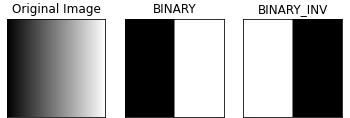
\includegraphics[width=11cm]{images/binary_threshold.jpg}
	\caption{Binarni threshold}
	\label{fig:binary_example}
\end{figure}
\\
\\
"Threshold" funkciju primjenjujemo na "grayscale" formatu ulazne slike. "Grayscale" je format u kojem pohranjujemo vrijednosti svakog piksela na ljestvici razine sivog odnosno od 0-255, gdje 0 predstavlja crni piksel a 255 bijeli. Jedan od ulaznih parametara "Threshold" funkcije je vrijednosna granica kojom odlučujemo pretvaramo li određeni piksel u crnu ili bijelu boju, ako je vrijednost piksela manja ili jednaka navedenoj granici piksel postaje crn a ako je iznad granice postaje bijel.


\begin{figure}[htb]
	\centering
	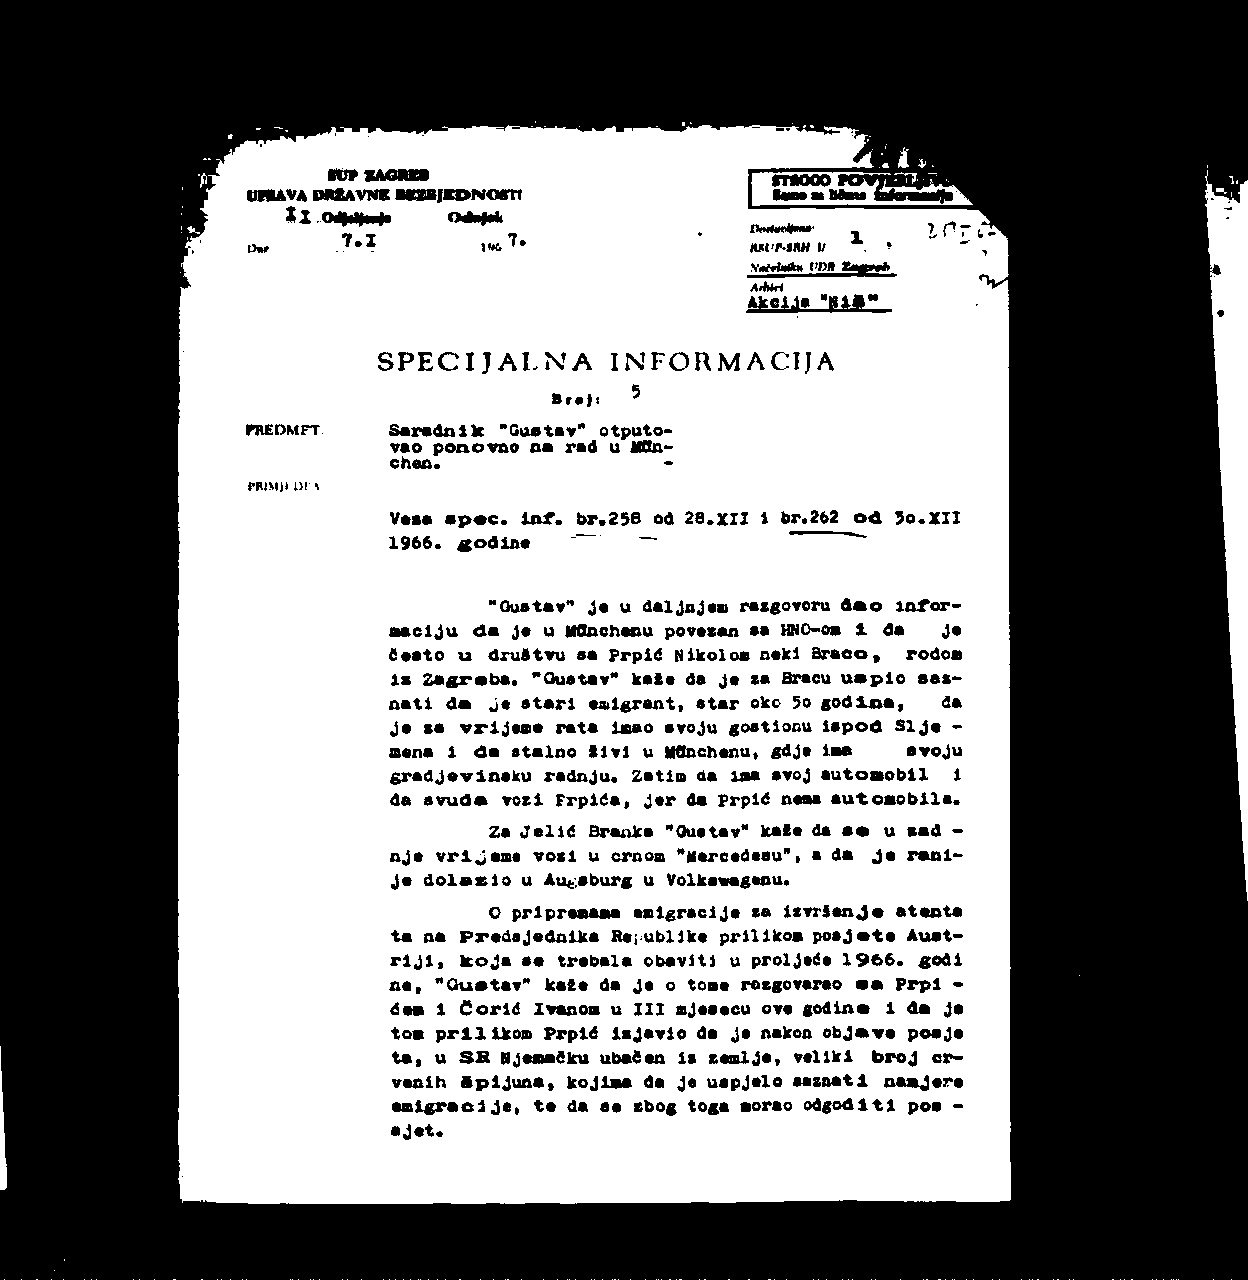
\includegraphics[width=10cm]{images/dataset_binary.jpg}
	\caption{Binarni threshold na primjeru materijala}
	\label{fig:dataset_binary_example}
\end{figure}

Nakon kreiranja binarne slike provodimo ju kroz detekciju ravnih linija odnosno koristimo "Hough Line Transform"\cite{hough}. Metoda "Hough Line Transform" popularna je metoda u područjima računalog vida i pretprocesiranja slika za detekciju ravnih linija na slici. Razvio ju je Paul Hough 1960-ih godina. "Hough Line Transform" radi tako da kartezijeve koordinate pretvorimo u parametarski prostor, još poznat kao "Hough space". U takvom parametarskom prostoru proces detekcije ravnih linija je olakšan jer linija prikazane formulom y=mx +c, gdje "m" označava nagib pravca i "c" sjecište sa ordinatom prikazujemo parametrima kuta i udaljenosti od ishodišta. Ovime izbjegavamo slučajeve u kojima nagib pravca nije definiran odnosno vertikalnih pravaca.
\\
Također "Hough Line Transform" otporan je na prisutni šum slike ili pojavljivanje prekidnih linija. Prekidne linije odnosno funkcije detektiramo tako da kroz pojedinu točku provodimo sve moguće linije i agregacijom svih linija detektiramo željenu odnosno prekidnu liniju.

\begin{figure}
\centering
    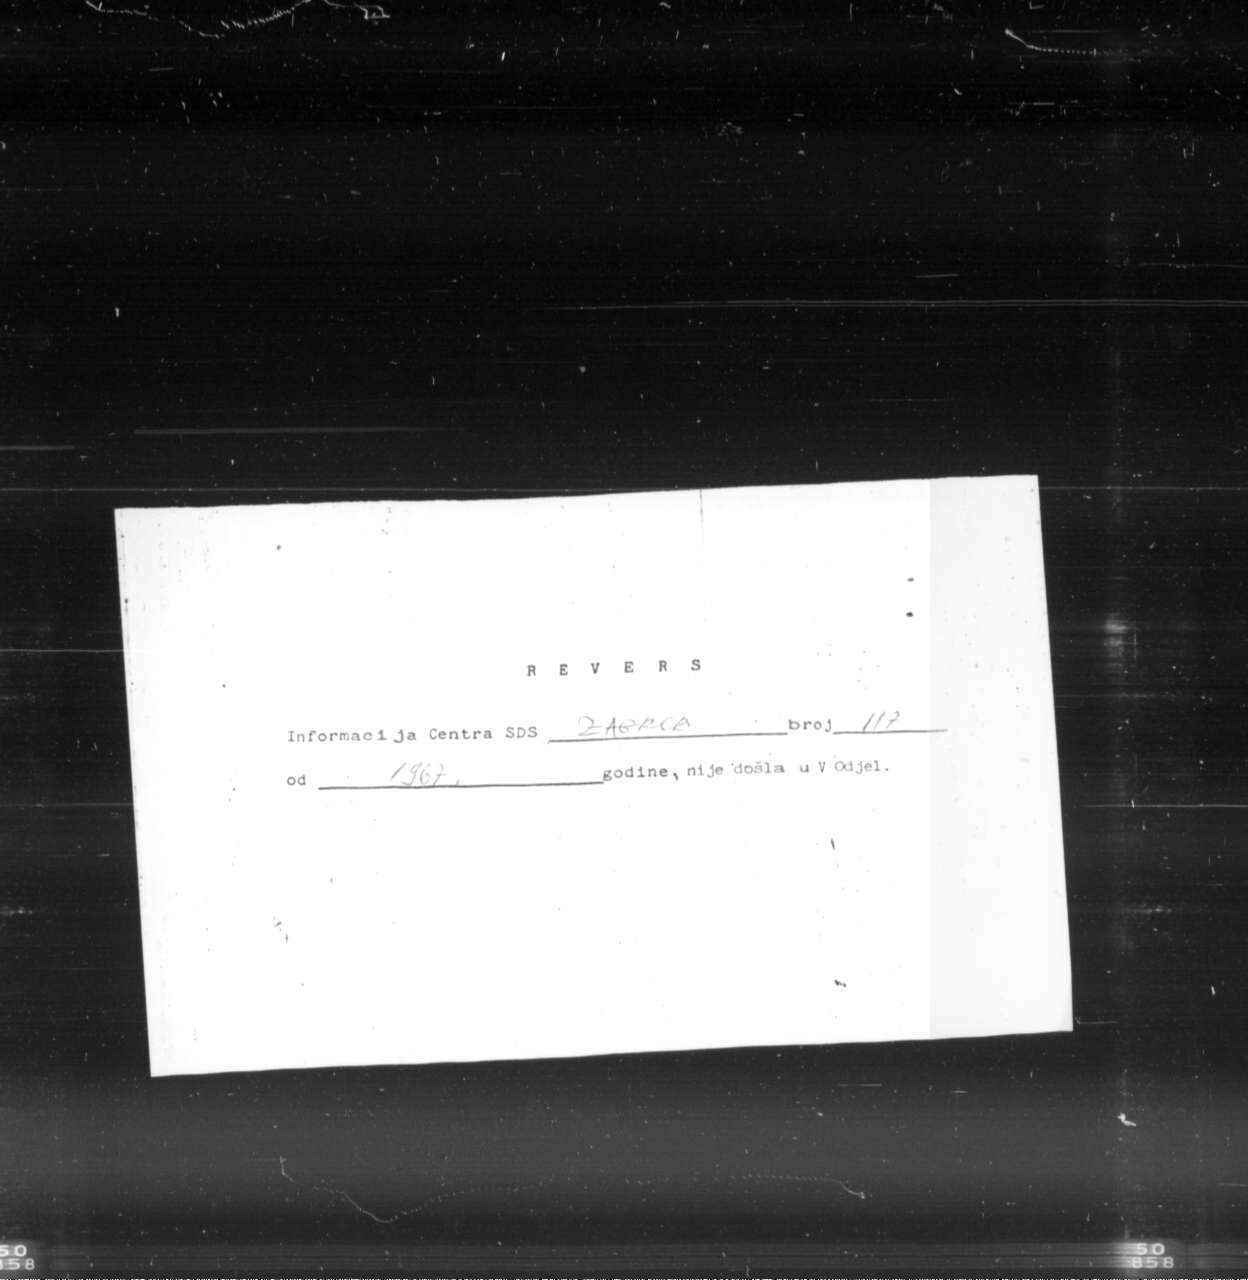
\includegraphics[width=11cm]{images/Z05353721.jpg}
    
\includegraphics[width=11cm]{images/Z05353721_draw.jpg}
    \caption{Korištenje Hough line transformacije (prije-gore, nakon-dolje)}
    \label{fig:houghline}
\end{figure}
\pagebreak
\subsection{Rotacijska funkcija}
Nakon detekcije ravnih linija u procesu obrade sljedeći korak je funkcija izračuna kuta potrebnog za rotaciju slike u željeni odnosno ispravni položaj. Ovaj korak krucijalan je jer kako bi dobili što bolje rezultate sustava za optičko prepoznavanje znakova moramo mu predati slike što sličnije onima na kojima je treniran. Ovaj problem se pojavljuje kod dokumenata koji su skenirani pod raznim kutevima i time je tekst na dokumentu zakrivljen za neku vrijednost.
\\
\\
Računanjem kuta rotacije skreniranog dokumenta i kasnije njegovim rotiranjem postižemo skup podataka koji su korak sličniji onima na kojima je sustav prepoznavanja znakova treniran i time postižemo bolje rezultate u prepoznavanju teksta i njegovom isčitavanju.
Kut rotacije računamo na način da od pronađenih linija napravimo manji skup linija kojima nagib je vrijednosno blizak osi ordinata i odabiremo vrijednost nagiba sa najučestalijim ponavljanjem. Kut nagiba s obzirom na os ordinata računamo korištenjem tangens funkcije.

Izračunom i odabirom kuta rotacija slike prolaze kroz "deskew" funkciju odnosno proces rotacije. Slike rotiramo s obzirom na njihovu točku središta za dobiveni kut rotacija i time dobivamo ispravno rotiranu sliku.
\\
\\
Kranji rezultat ovog koraka su ispravno rotirane slike na kojima je sadržaj odnosno tekst horizontalan.
\\

\begin{figure}[H]
\centering
    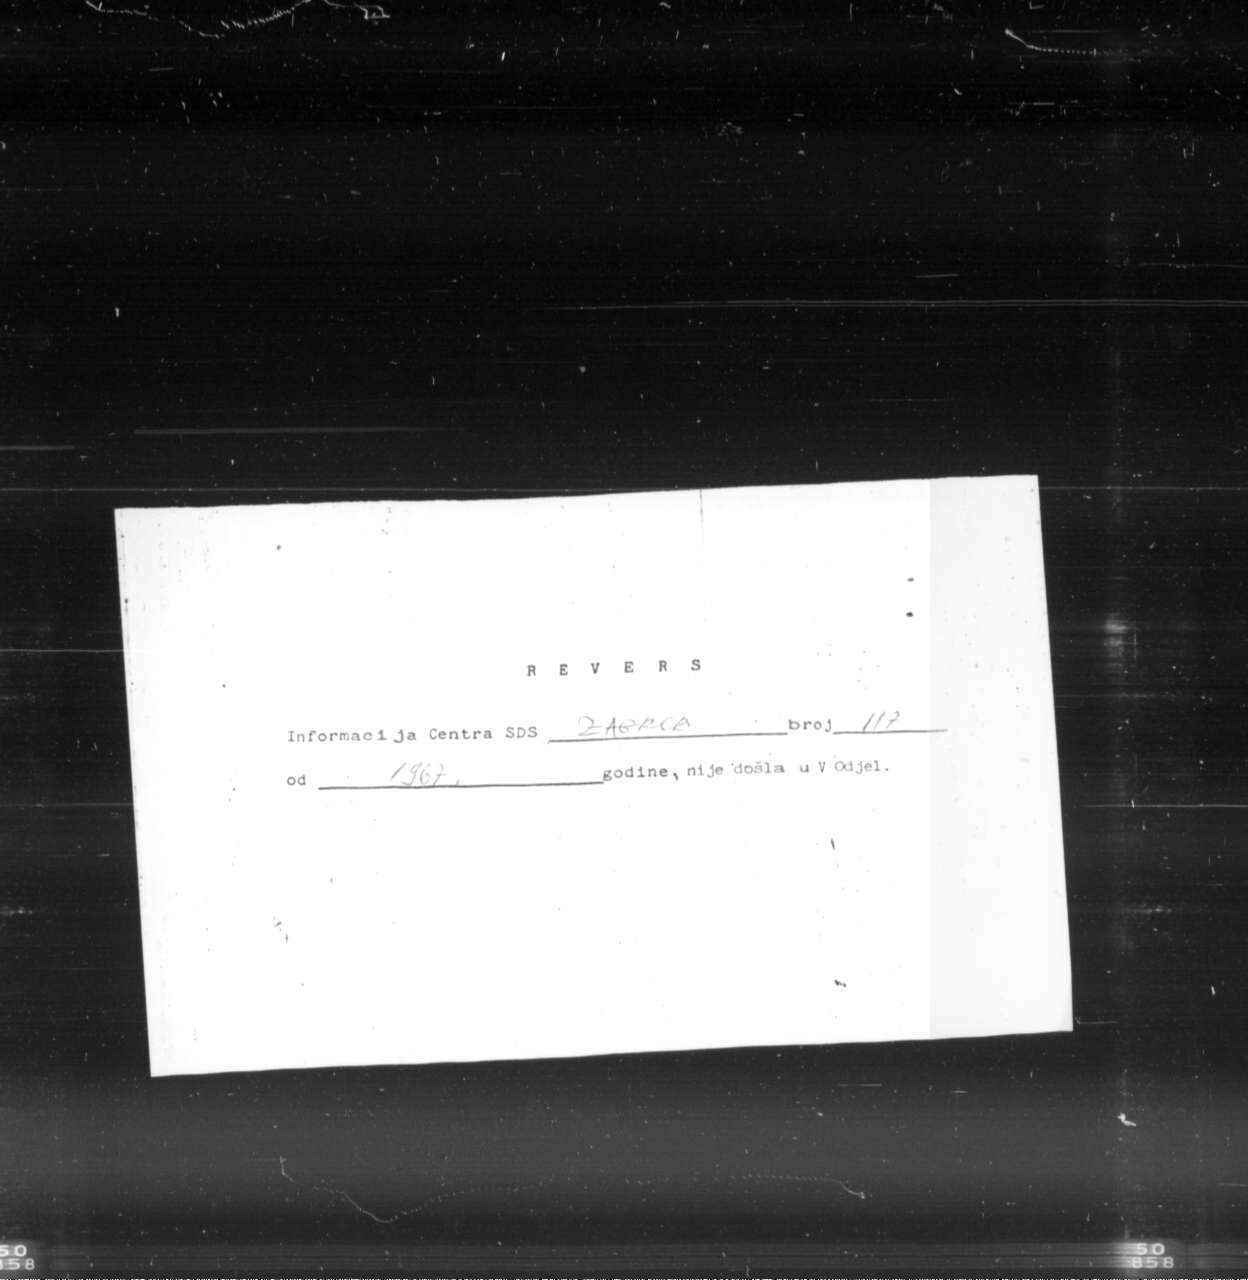
\includegraphics[width=11cm]{images/Z05353721.jpg}
    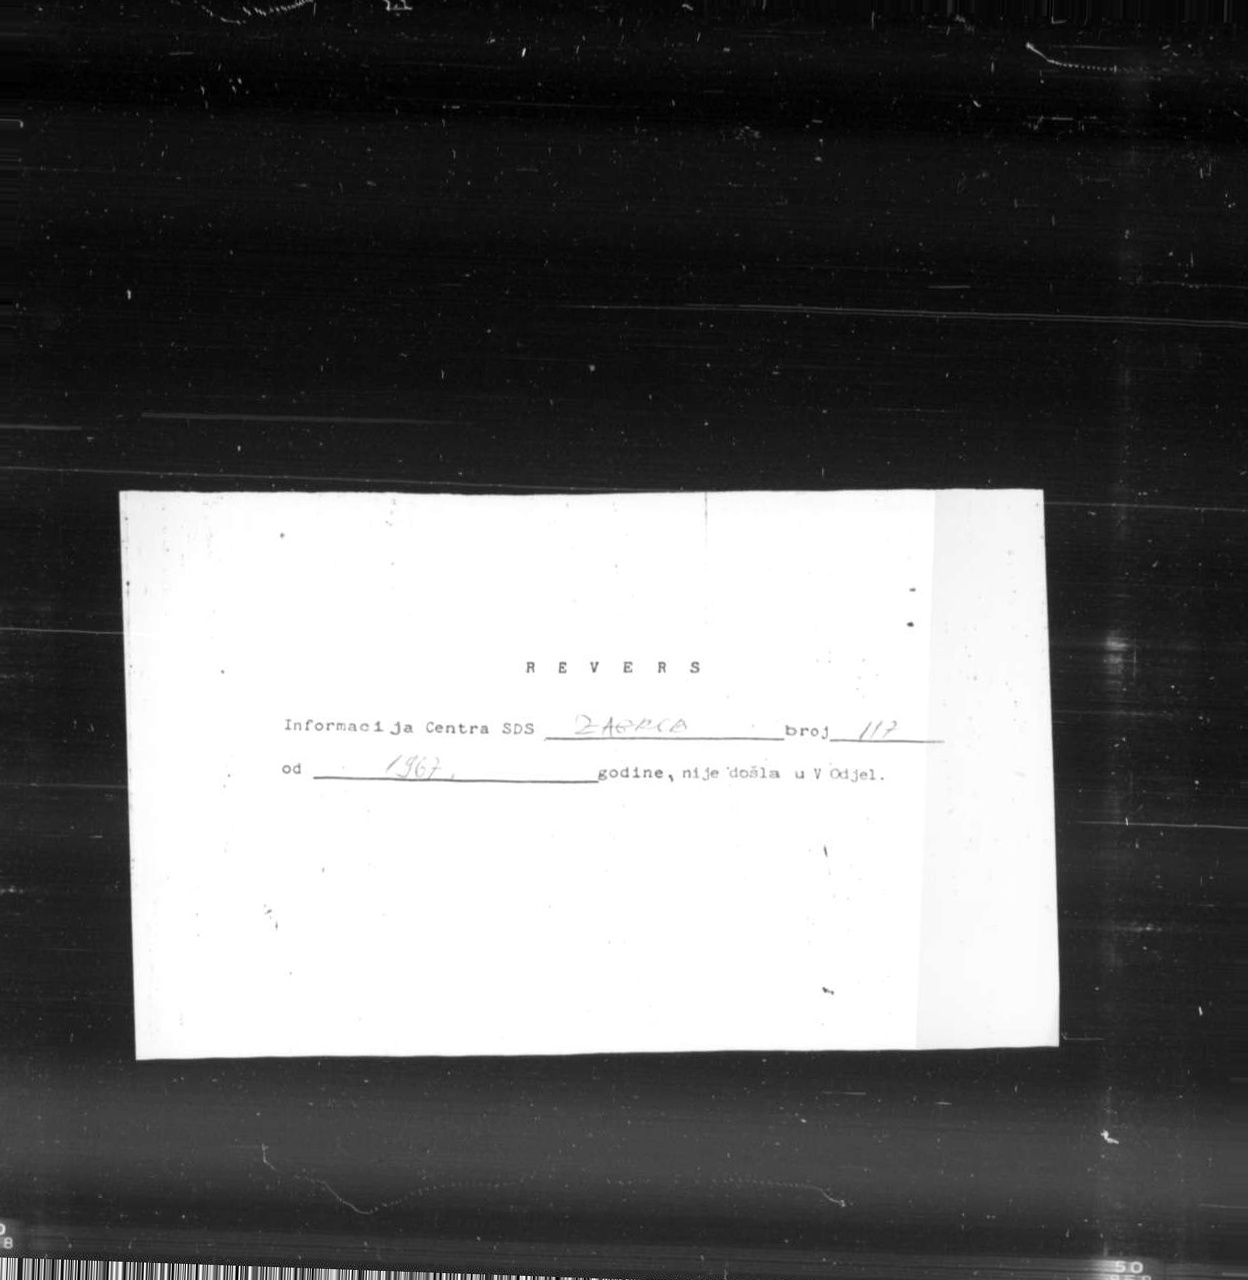
\includegraphics[width=11cm]{images/Z05353721_deskewed.jpg}
    \caption{Primjer rezultata metode deskewed (prije-gore, nakon-dolje)}
	\label{fig:example_deskewed}
\end{figure}
\pagebreak
\subsection{Prepoznavanje obrisa}
U skupu podataka nailazimo na slike skeniranih dokumenata različitih dimenzija, oblika papira pa čak i slike na kojima su dostupni više od jednog dokumenta. Naime u nekoliko slučajeva sliku mogu činiti više od jednog dokumenta čime je jedan prisutan u cijelosti a drugog dokumenta vidimo ili dio stranice ili rub stranice. Ovdje nailazimo na problem prepoznavanje dokumenta od značaja. Pretpostavimo li da dokument koji gledamo je uvijek u cijelosti ili većinski prisutan na slici od drugog dokumenta koji se pojavljuje, možemo zaključiti da će njegova površina uvijek biti veća od drugog dokumenta. Izračun površine prisutnih dokumenata na slici provodimo procesom "Contour detection"\cite{contour}. 
\\
\hfill \break
Neke mogućnosti procesa "Contour detection" su:
\begin{itemize}
  \item prepoznavanje objekata
  \item proces segmentacije 
  \item analiziranje i mjerenje oblika
  \item praćenje objekata
\end{itemize}
\hfill \break
U svrhu ovog rada koristimo mogućnosti prepoznavanja objekata, svih prisutnih dokumenata na slici, te analiziranje i mjerenje objekata odnosno računanje površine prisutnih dokumenata.
\begin{figure}[H]
\centering
    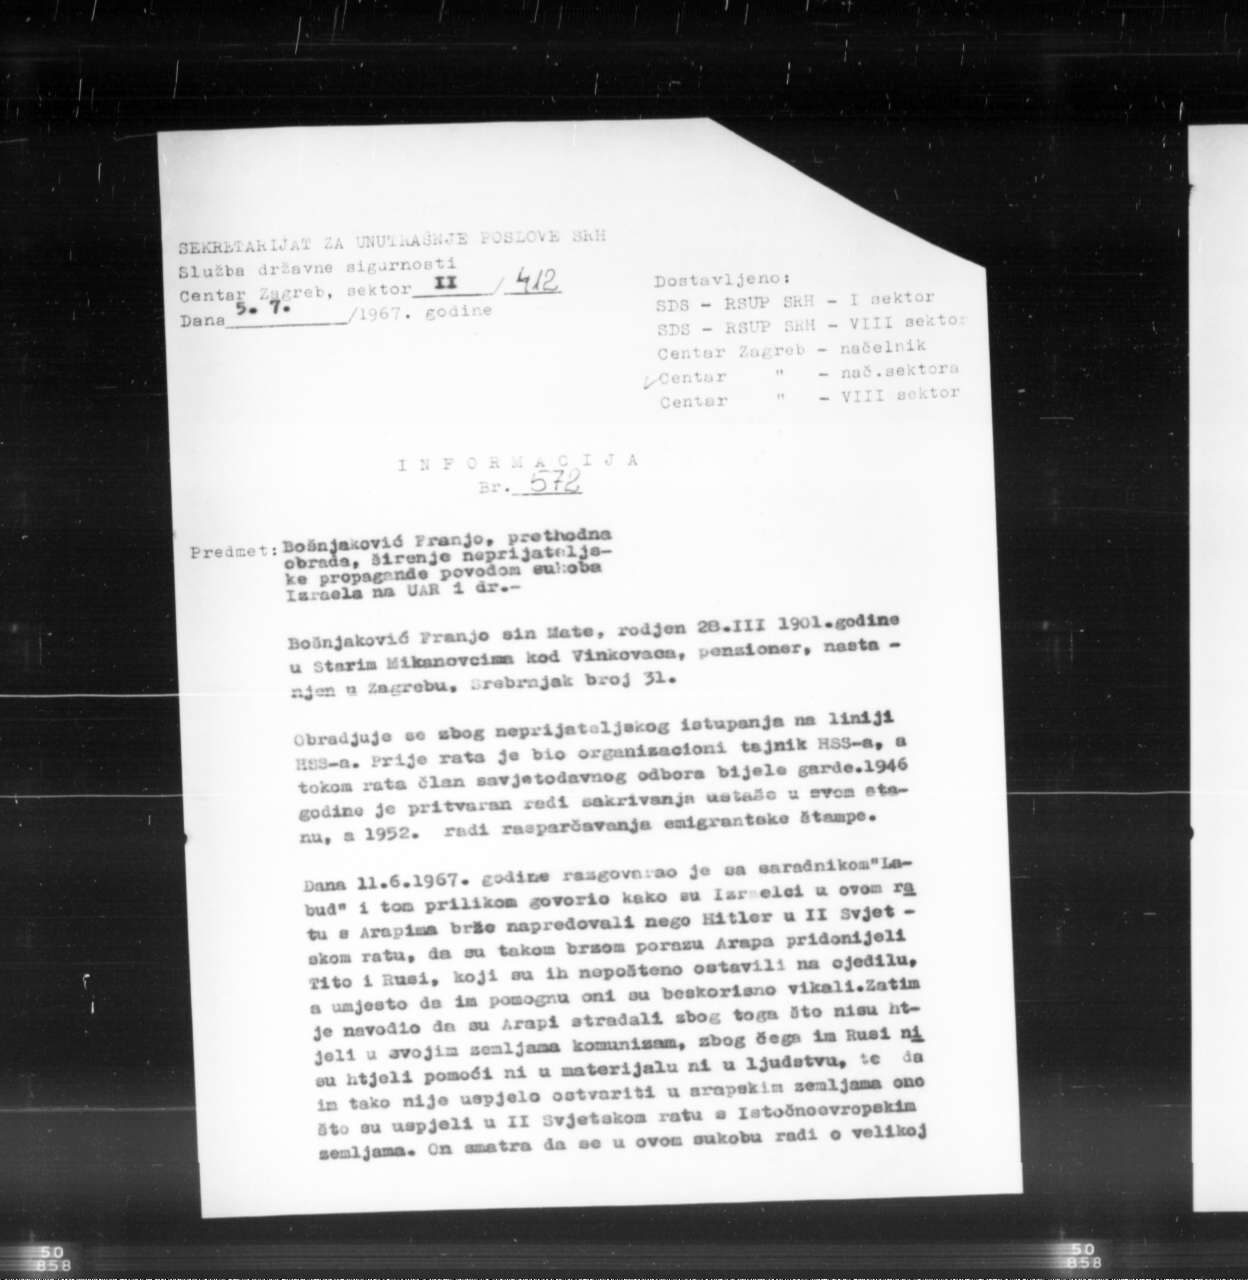
\includegraphics[width=7cm]{images/vise papira na jednoj slici.jpg}
    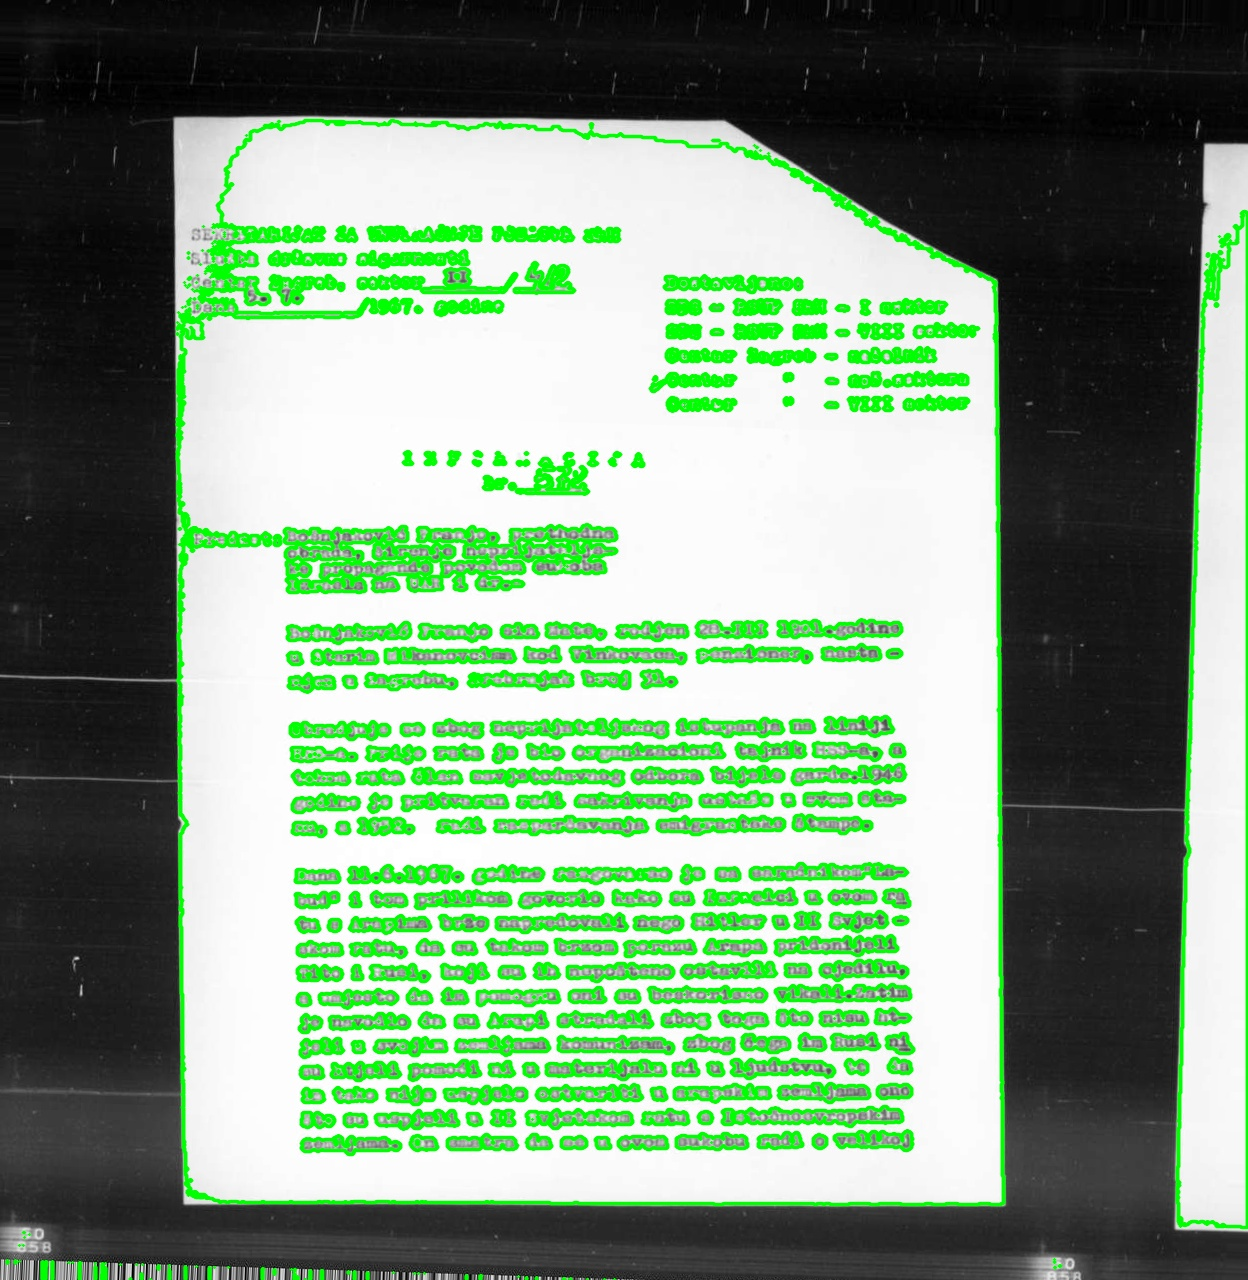
\includegraphics[width=7cm]{images/vise kontura nacrtane.jpg}
    \caption{Primjer primjene metode contour detection (lijevo-originalna slika, desno-pronaeni obrisi na originalnoj slici)}
	\label{fig:example_deskewed}
\end{figure}
\pagebreak
Nakon detekcije dokumenta od značaja, kreiramo četverokut oko pronađene konture dokumenta i kreiramo novu sliku koju čini isključivo dokument od značaja.
\\
\begin{figure}[H]
    \centering
    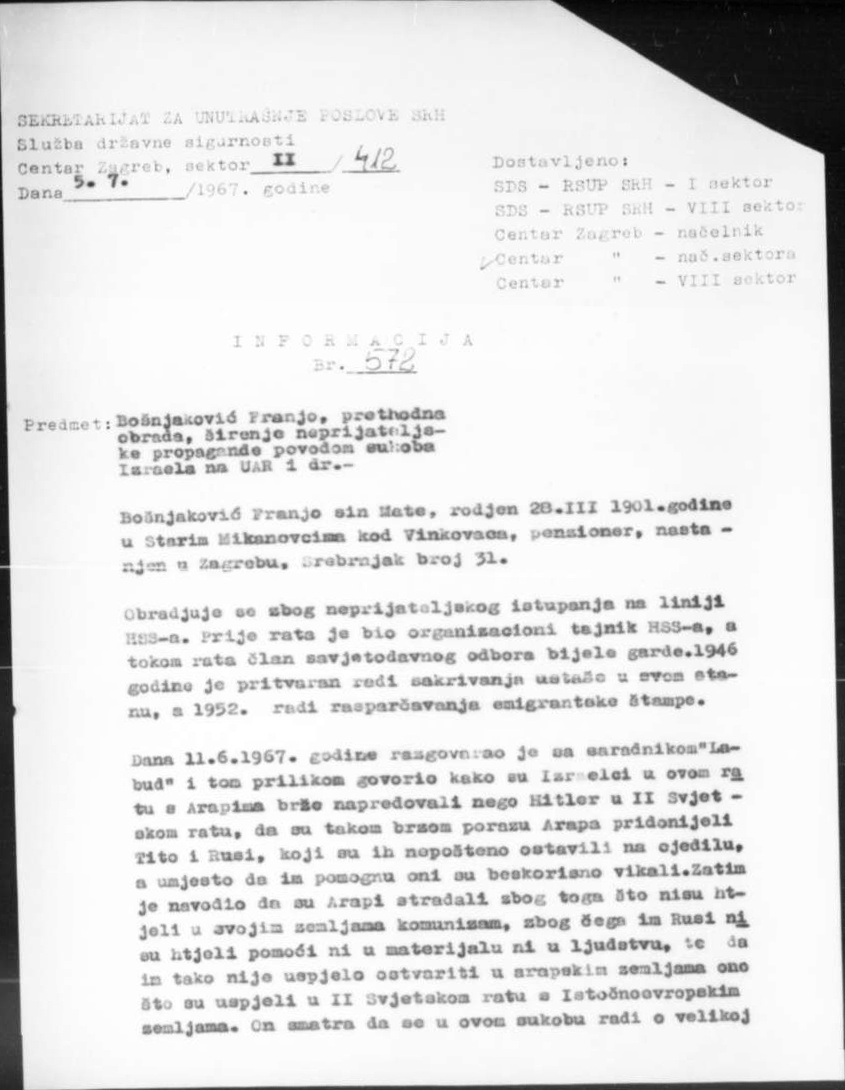
\includegraphics[width=10cm]{images/vise kontura max slika.jpg}
    \caption{Primjer slike nakon metode contour}
	\label{fig:example_deskewed}
\end{figure}

\subsection{Povećanje rezolucije slika}
Kako bi dodatno poboljšali rezultate optičkog prepoznavanja koristimo metodu poboljšanja rezolucije i kvalitete ulaznog podatka. Primjenom ove metode povećavamo broj piksela u slici i time postižemo detaljniju i kvalitetniju sliku za kasniju obradu. Uvećanjem rezolucije postižemo dokumente koji sadrže čitljiviji tekst, povećanjem oštrine i jasnoće, manje šuma i povećavamo razmak između znakova unutar teksta. S navedenim svojstvima postižemo precizniju interpretaciju i klasifikaciju znakova.

U ovom radu koristimo predtrenirani model uveličanja rezolucije slike "FSCRNN" odnosno "Fast Super-Resolution Convolutional Neural Network". Ovaj model koristi metodu dubukog učenja kako bi postigao sliku visoke rezolucije i kvalitete iz slike niske rezolucije.

\subsection{Adaptive threshold}
Načinu rješavanja problema različite razine osvjetljenja teksta možemo pristupiti već navedenom metodom "Binary Threshold" kojom lakše raspoznajemo dokument odnosno papir i tekst na dokumentu. Do problema dolazi zbog različitih razina osvjetljenja. Naime pikseli koji čine jedan dio teksta imaju više razine sivog od ostatka teksta na slici i time se klasificiraju u bijeli piksel dok ostali u crni piksel. Time dolazi do gubitka podataka na krajnjem rezultatu, kako bi ti izbjegli koristimo drugu metodu "threshold-a", "Adaptive Threshold"\cite{OpenCVadaptive}. Glavna prednost "Adaptive Threshold" metode je podjela ulaznog podataka na manje regije i pojedinačna analiza svake regije s obzirom na pripadna svojstva.

Vrijednost "threshold-a" određujemo uporabom "Gaussian Adaptive Threshold" varijante u kojoj vrijednost određujemo tako da računamo prosjek inteziteta piksela u regiji te pikselima bližim sredini regije dodjeljujemo više težinske vrijednosti a pikselima bliže ruba regije niže. Računamo prosjek težinskih vrijednosti piksela u regiji i određeni prosjek predstavlja nam lokalnu vrijednost "threshold-a". Kao i u "Binary Threshold" metodi svi pikseli čija težinska vrijednost je veća od lokalne vrijednosti klasificiramo kao bijeli piksel a ostale crni. Ovaj proces provodimo za sve podijeljene regije.
\pagebreak
\begin{center}
\begin{minipage}{0.48\linewidth}
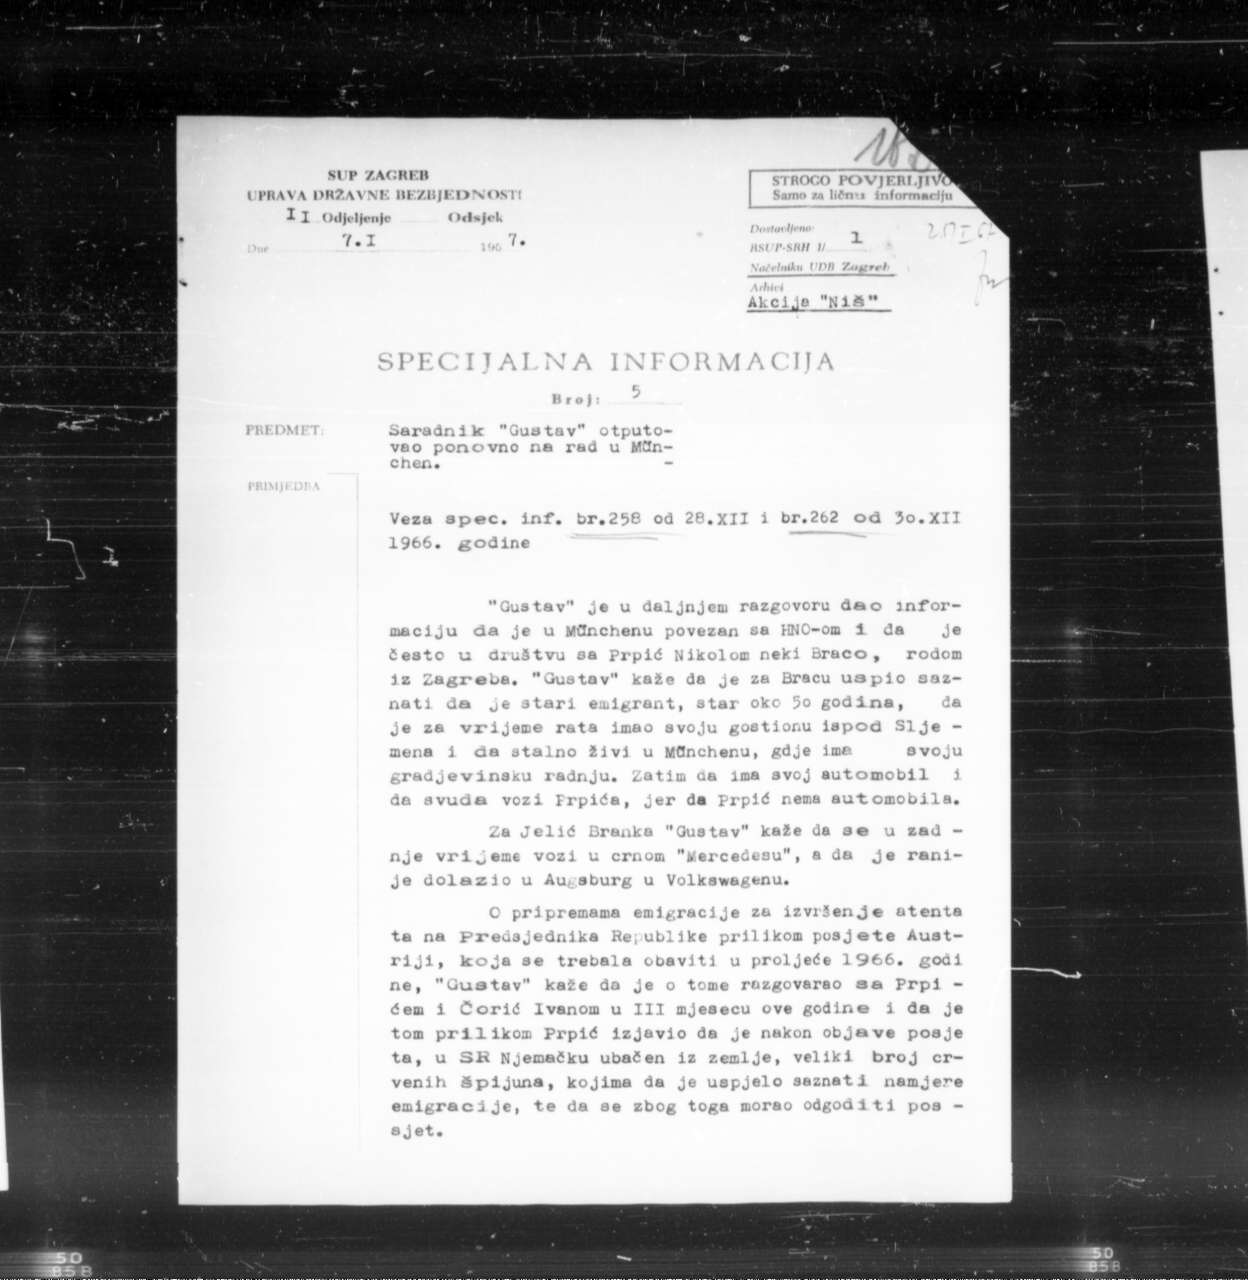
\includegraphics[width=6cm]{images/thresh/Z05353422.jpg}
\captionof{figure}{Primjer originalne slike}
\end{minipage}%
\hfill
\begin{minipage}{0.49\linewidth}
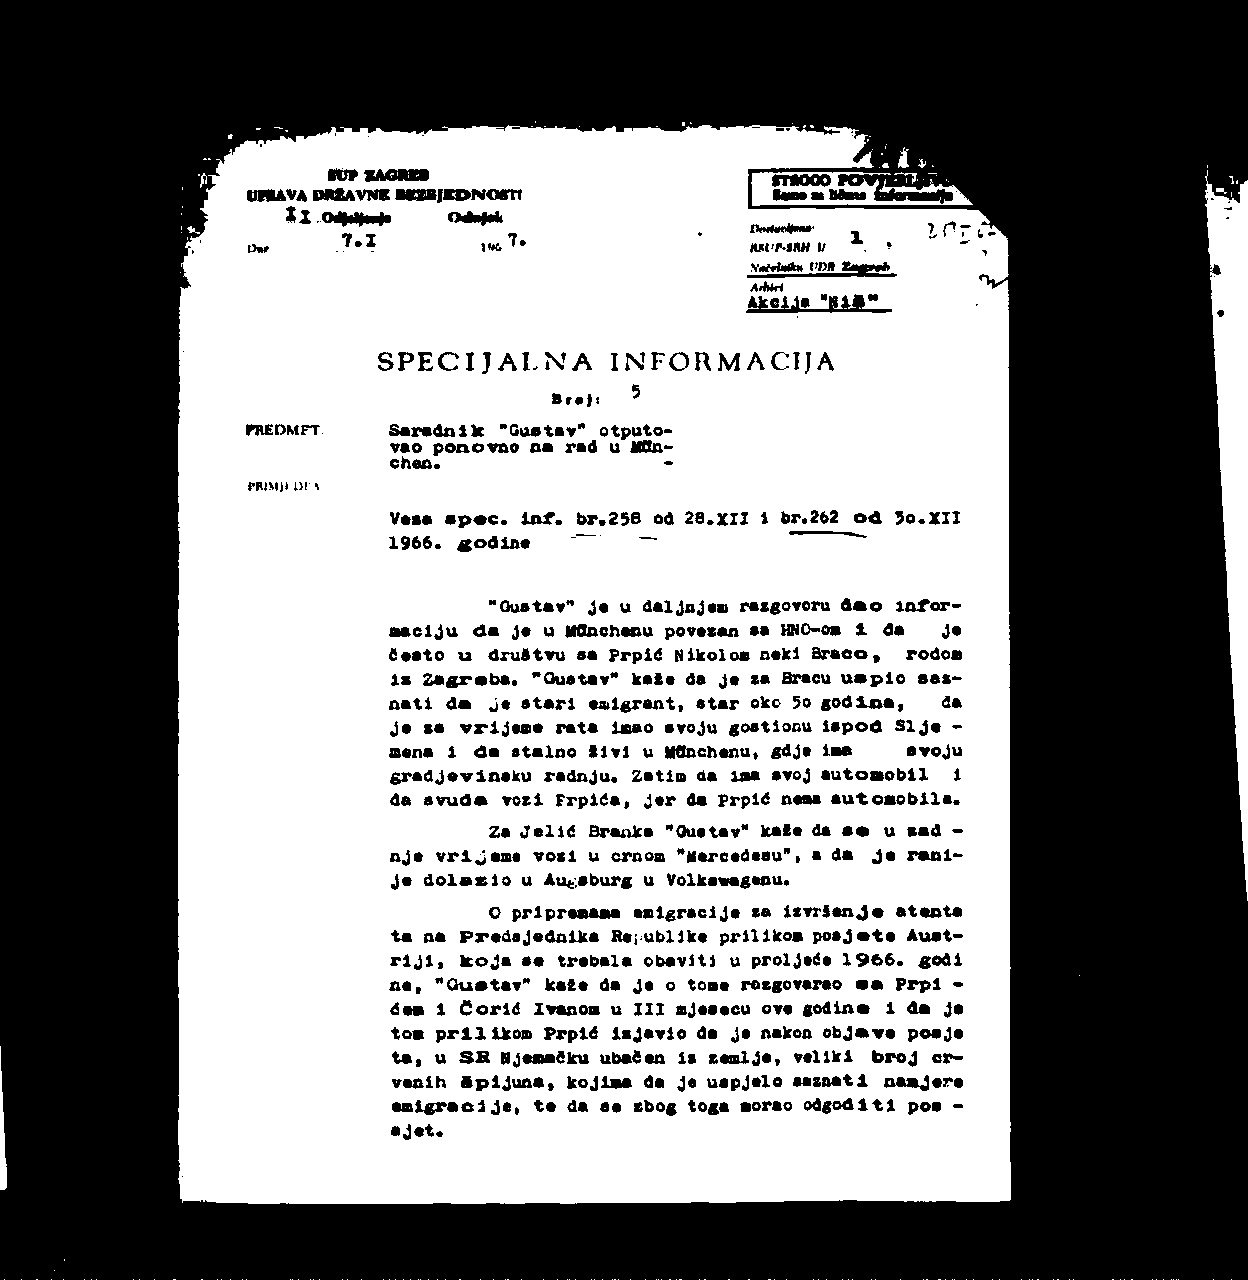
\includegraphics[width=6cm]{images/thresh/Z05353422_thresh.jpg}
\captionof{figure}{Binary threshold}
\end{minipage}
\end{center}
\begin{center}
\begin{minipage}{0.49\linewidth}
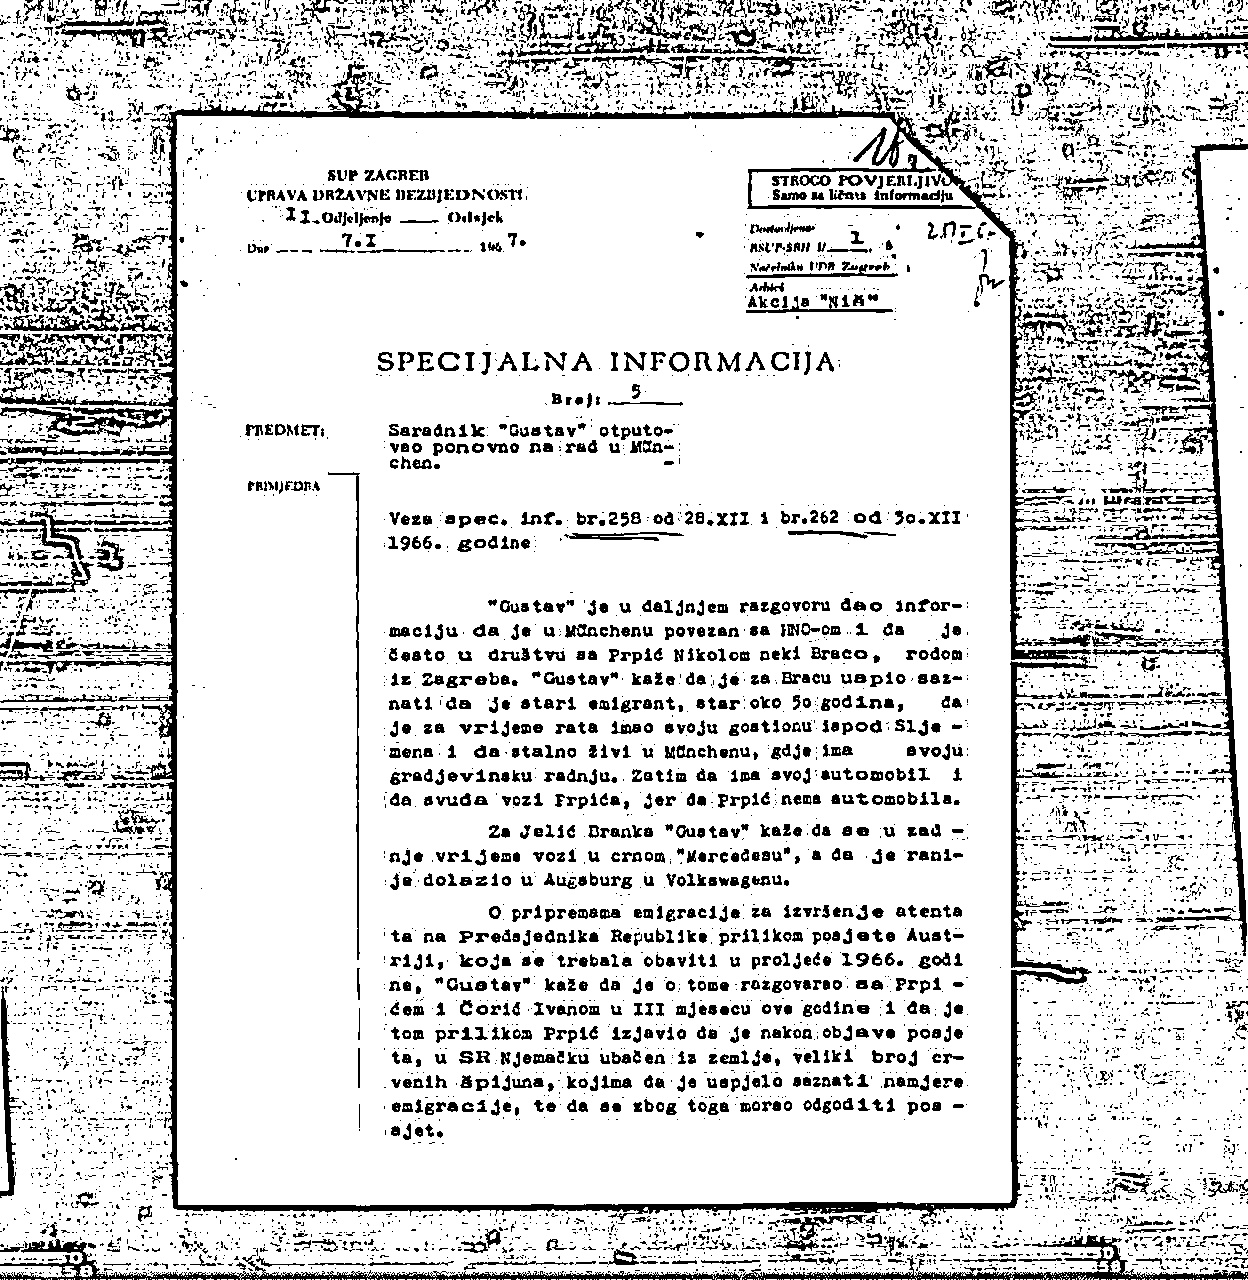
\includegraphics[width=6cm]{images/thresh/Z05353422_thresh_mean.jpg}
\captionof{figure}{Adaptive threshold mean}
\end{minipage}
\hfill
\begin{minipage}{0.49\linewidth}
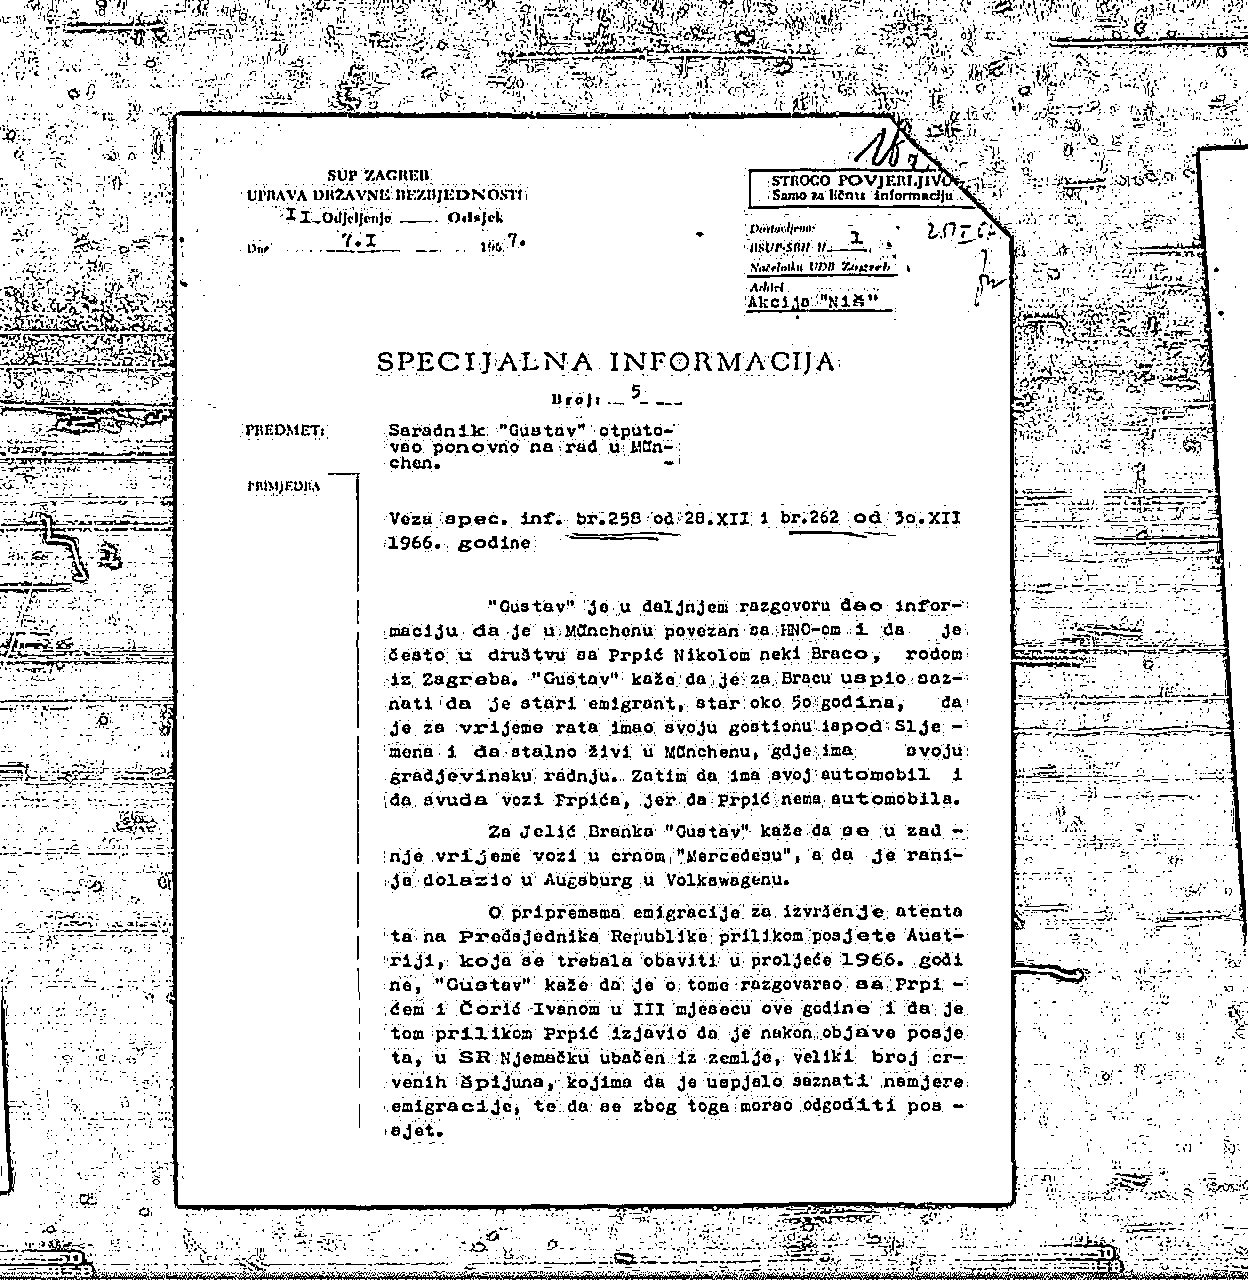
\includegraphics[width=6cm]{images/thresh/Z05353422_thresh_gauss.jpg}
\captionof{figure}{Adaptive threshold Gaussian}
\end{minipage}
\end{center}

\subsection{Stanjivanje fonta i zamućenje}
U ovom koraku primjenjujemo metode stanjivanja fonta odnosno "thin font" i zamućenja slika uoprabom metode "blur" kako bi poboljšali rezultate optičkog prepoznavanja znakova na ulaznim podatcima. Preciznije "thin font" metodom stanjujemo font prisutan na dokumentima i time postižemo neke od značajki:
\hfill \break
\begin{itemize}
  \item povećani razmak između znakova
  \item jasnije rubove znakova
  \item smanjenje šuma
\end{itemize}
\hfill \break
U svrhu ovog rada od značaja je povećanja razmaka i postizanja jasnijih rubova.
\\
Stanjivanjem fonta smanjujemo površinu koju zauzimaju znakovi na dokumentu odnosno povećavamo razmak znaka od ostalih znakova. Time postižemo lakše prepoznavanje svih prisutnih znakova na dokumentu.
\\
Postizanjem jasnijih rubova oko pristunih znakova također poboljšavamo lakše prepoznavanje znakova te smanjenje prisutnog šuma.

Smanjenje šuma također postižemo i primjenom metode "blur" na cjeloviti dokument. Za svaki piksel prisutan na ulaznom podatku računamo prosječnu vrijednost piksela s obzirom na njegove susjede. Time postižemo zaglađivanje piksela i piksele koji predstavljaju šum na slici normaliziramo sa susjednim pikselima. Time postižemo rezultate s manjom količinom šuma i u konačnici podatke koji su lakše čitljiviji sustavu za prepoznavanje znakova.

\section{Optičko prepoznavanje znakova}
Optičko prepoznavanje podataka je tehnologija koja omogućuje računalima prepoznavanje i interpretiranje isprintanog ili rukom pisanog teksta na slikanim ili skeniranim dokumentima. Ovakav način obrade podataka pronalazi široku upotrebu u raznim područjima kako bi ubrzali procese obrade, prepoznavanje teksta i digitalizacije starih dokumenata.
U ovom radu primjena optičkog prepoznavanja podataka korištena je za prepoznavanje i isčitavanja podataka sa stare arhivske dokumentacije.

\subsection{Tesseract}
U ovom radu koristimo sustav optičkog prepoznavanje znakova "Tesseract" odnosno njegovu inačicu za programski jezik python "pytesseract". Nakon što je proces obrade slike gotov i dobili smo krajnji rezultat pretprocesiranja, te podatke prosljeđujemo sustavu "Tesseract" koji nad tim podatcima provodi prepoznavanje i interpretiranje znakova te stvara krajnju tekstualnu datoteku pronađenog teksta. 
\\

Sustav "Tesseract" nudi različite opcije rada kojima definiramo koji način segmentacije koristiti. Definiranjem načina segmentacije odnosno kakve ulazne podatke da očekuje, dobivamo preciznije rezultate prepoznavanje i time krajnje rezultate.
Neke od metoda segmentacije koje sustav "tesseract" omogućuje su: 
\hfill \break
\begin{itemize}
  \item Orientation and script detection (OSD) only
  \item Assume a single uniform block of vertically aligned text
  \item Assume a single uniform block of text
  \item Treat the image as a single text line
  \item Treat the image as a single word
  \item Treat the image as a single character
\end{itemize}
\hfill \break
Metodu segmentacije koju koristimo je "Assume a single uniform block of vertically aligned text" jer najpreciznije definira ulazne podatke koji su nam dostupni a to su blokovi teksta koji su vertikalno usklađeni. Također tu primjećujemo značaj koraka pretprocesiranja u kojem nam je rezultat bio skenirani dokument sa blokovima teksta koji su vertiklano usklađeni. Mogli smo koristiti i ostale metode segmentacije ali onda bi trebali koristiti i drugačiji način pretprocesiranja kako bi sustavu omogućili što vjernije podatke onima na kojima je treniran.

Osim metode segmantacije sustav "tesseract" omogućuje i definiranje jezika na kojem je tekst pisan. Time pospješuje prepoznavanje znakova koji su dio nekog jezika te riječi koje čine taj jezik. Ulazni podatci pisani su hrvatsko-srpskim jezikom, "tesseract" ne podržava navedeni jezik stoga smo koristili kombinaciju hrvatskog i srpskog jezika(latnice).

%ubaci tablicu ako nije definiran jezik i ako je
\subsection{OCR metrike}
Kako bi lakše pratili koje metode obrade i optičkog prepoznavanje pružaju preciznije krajnje rezultate koristimo metriku "CER"\cite{CER} optičkog prepoznavanja. "CER" ili "Character method rate" je metrika optičkog prepoznavanja podataka kojom računamo koliko precizno je sustav prepoznao i interpretirao ulazne podatke. Vrijednost preciznosti postižemo izračunom brojem znakova koja smo uklonili, dodali ili izmjenili iz rezultata optičkog prepoznavanja kako bi dobili početnu riječ.

\chapter{Rezultati}
U nastavku su prikazani rezultati optičkog prepoznavanja znakova uz korištenje raznih metoda koje pridonose postizanju preciznijih rezultata.

\subsection{Korištenje metode zamućenja}
Korištenjem metode blur postižemo globalno zaglađenje prisutnih znakova na skeniranom dokumentu. Ovom metodom smanjujemo šum oko znakova i postižemo preciznije rezultate prepoznavanja znakova. U sljedećim tablicama jačina korištene metoda interpretirana je oznakom "blur 0, 5, 10". "blur 0" označava ne korištenje metode blur. Najpreciznije rezultate postižemo korištenjem metode "blur 5" koja predstavlja lagano zaglađivanje znakova. U konačnici, korištenjem metode blur očekujemo i postižemo bolje rezultate ali također korištenjem prejakog zaglađivanja gubi se preciznost i točnost interpretiranja znakova.
\begin{table}[H]
	\caption{Rezultati korištenjem razine "blur 0"}
	\label{tbl:Blur 0}
 \centering
        \begin{tabular}{ |*{4}{c|} } \hline
	\multicolumn{1}{|c|}{Slika} & \multicolumn{1}{|c|}{Očekivano} & \multicolumn{1}{|c|}{Pronađeno} & \multicolumn{1}{|c|}{CER}\\ \hline
Z05353721&20&5&0.094545\\ \hline
Z05353668&279&137&0.396187\\ \hline
Z05353422&212&146&0.236147\\ \hline
Z05353778&157&103&0.394797\\ \hline
Z05353396&165&121&0.332736\\ \hline
Z05353424&269&160&0.274321\\ \hline
Z05353401&169&101&0.415124\\ \hline
Z05353836&127&85&0.358741\\ \hline
Z05353758&116&79&0.240498\\ \hline
Z05353673&121&78&0.418628\\ \hline
	\end{tabular}
\end{table}


\begin{table}[H]
	\caption{Rezultati korištenjem razine "blur 5"}
\label{tbl:Blur 2}
\centering
        \begin{tabular}{ |*{4}{c|} } \hline
	\multicolumn{1}{|c|}{Slika} & \multicolumn{1}{|c|}{Očekivano} & \multicolumn{1}{|c|}{Pronađeno} & \multicolumn{1}{|c|}{CER}\\ \hline
Z05353721&20&6&0.063636\\ \hline
Z05353668&279&147&0.420519\\ \hline
Z05353422&212&146&0.228544\\ \hline
Z05353778&157&103&0.370627\\ \hline
Z05353396&165&126&0.32723\\ \hline
Z05353424&269&164&0.286411\\ \hline
Z05353401&169&101&0.433214\\ \hline
Z05353836&127&81&0.368691\\ \hline
Z05353758&116&83&0.235522\\ \hline
Z05353673&121&74&0.410493\\ \hline
	\end{tabular}
\end{table}

\begin{table}[H]
	\caption{Rezultati korištenjem razine "blur 10"}
        \label{tbl:Blur 2}
        \centering
        \begin{tabular}{ |*{4}{c|} } \hline
	\multicolumn{1}{|c|}{Slika} & \multicolumn{1}{|c|}{Očekivano} & \multicolumn{1}{|c|}{Pronađeno} & \multicolumn{1}{|c|}{CER}\\ \hline
Z05353721&20&7&0.106926\\ \hline
Z05353668&279&139&0.401832\\ \hline
Z05353422&212&138&0.254155\\ \hline
Z05353778&157&102&0.385322\\ \hline
Z05353396&165&122&0.345172\\ \hline
Z05353424&269&162&0.321551\\ \hline
Z05353401&169&103&0.42685\\ \hline
Z05353836&127&84&0.361008\\ \hline
Z05353758&116&82&0.246549\\ \hline
Z05353673&121&70&0.381782\\ \hline
	\end{tabular}
\end{table}

\subsection{Definiranje jezika materijala}
U nastavku su pikazani rezultati prepoznavanja podataka nad jednakim ulaznim podatcima sa razlikom definicije jezika na kojem su skenirani dokumenti pisani. Tablica 5.4. prikazuje rezultate nakon definiranog jezika "hrvatski + srpski" dok tablica 5.5. prikazuje bez definiranog jezika. Za uočiti je da rezultati ne prikazuju konzinstentan napredak definicijom korištenog jezika. Razlog tome je što jezik kojim su skenirani dokumenti pisani nije podržan od strane Tesseract-a i kombinacija hrvatsko srpskog jezika ne predstavlja najvjerniju zamjenu.
\begin{table}[H]
	\caption{Rezultati definiranjem jezika}
        \label{tbl:Blur 2}
        \centering
        \begin{tabular}{ |*{4}{c|} } \hline
	\multicolumn{1}{|c|}{Slika} & \multicolumn{1}{|c|}{Očekivano} & \multicolumn{1}{|c|}{Pronađeno} & \multicolumn{1}{|c|}{CER}\\ \hline
Z05353721&20&6&0.078787\\ \hline
Z05353668&279&149&0.416695\\ \hline
Z05353422&212&146&0.228544\\ \hline
Z05353778&157&103&0.382869\\ \hline
Z05353396&165&120&0.312126\\ \hline
Z05353424&269&167&0.290048\\ \hline
Z05353401&169&107&0.416096\\ \hline
Z05353836&127&81&0.3686907\\ \hline
Z05353758&116&80&0.2250678\\ \hline
Z05353673&121&71&0.3755202\\ \hline
	\end{tabular}
\end{table}

\begin{table}[H]
	\caption{Rezultati ne definiranjem jezika}
        \label{tbl:Blur 2}
        \centering
        \begin{tabular}{ |*{4}{c|} } \hline
	\multicolumn{1}{|c|}{Slika} & \multicolumn{1}{|c|}{Očekivano} & \multicolumn{1}{|c|}{Pronađeno} & \multicolumn{1}{|c|}{CER}\\ \hline
Z05353721&20&7&0.127056\\ \hline
Z05353668&279&157&0.402159\\ \hline
Z05353422&212&148&0.236061\\ \hline
Z05353778&157&102&0.387575\\ \hline
Z05353396&165&119&0.312746\\ \hline
Z05353424&269&167&0.285546\\ \hline
Z05353401&169&107&0.424054\\ \hline
Z05353836&127&85&0.3702583\\ \hline
Z05353758&116&82&0.2272948\\ \hline
Z05353673&121&69&0.3692015\\ \hline
	\end{tabular}
\end{table}

\subsection{Provođenje prepoznavanja znakova nad pretprocesiranim slikama i originalnim materijalima}
Tablice 5.6. i 5.7. prikazuju rezultate prepoznavanja znakova provodenih na originalnim slikama arhive i slikama koje su prošle proces pretprocesiranja. Dobiveni rezultati jasno prikazuju značaj metoda korištenih u pretprocesiranju slika.
\begin{table}[H]
	\caption{Rezultati korištenjem processed image}
        \label{tbl:Blur 2}
        \centering
        \begin{tabular}{ |*{4}{c|} } \hline
	\multicolumn{1}{|c|}{Slika} & \multicolumn{1}{|c|}{Očekivano} & \multicolumn{1}{|c|}{Pronađeno} & \multicolumn{1}{|c|}{CER}\\ \hline
Z05353721&20&6&0.0787878\\ \hline
Z05353668&279&149&0.416695\\ \hline
Z05353422&212&146&0.228544\\ \hline
Z05353778&157&103&0.382869\\ \hline
Z05353396&165&120&0.312126\\ \hline
Z05353424&269&167&0.290048\\ \hline
Z05353401&169&107&0.416096\\ \hline
Z05353836&127&81&0.3686907\\ \hline
Z05353758&116&80&0.2250678\\ \hline
Z05353673&121&71&0.3755202\\ \hline
	\end{tabular}
\end{table}

\begin{table}[H]
	\caption{Rezultati korištenjem not processed image}
        \label{tbl:Blur 2}
        \centering
        \begin{tabular}{ |*{4}{c|} } \hline
	\multicolumn{1}{|c|}{Slika} & \multicolumn{1}{|c|}{Očekivano} & \multicolumn{1}{|c|}{Pronađeno} & \multicolumn{1}{|c|}{CER}\\ \hline
Z05353721&20&0&100\\ \hline
Z05353668&279&0&100\\ \hline
Z05353422&212&1&0.72727\\ \hline
Z05353778&157&0&100\\ \hline
Z05353396&165&0&100\\ \hline
Z05353424&269&1&0.7\\ \hline
Z05353401&169&0&100\\ \hline
Z05353836&127&0&100\\ \hline
Z05353758&116&0&100\\ \hline
Z05353673&121&0&100\\ \hline
	\end{tabular}
\end{table}

\subsection{Korištenje metode Image upscale}
U nastavku tablicama 5.8. i 5.9. prikazanih su rezultati za slike niskih rezolucija naspram slika visokih rezolucija. Napredak korištenjem ove metode jasan je pogledamo li stupac "Pronađeno" u navedenim tablicama. Provođenjem prepoznavanja podataka nad slikama visokih rezolucija sustav je prepoznao više riječi nego nad slikama niske rezolucije. Vrijednost pogreške CER za neke slučajeve ostaje slična dok za neke primjećujemo jasan napredak. Iako u nekim slučajevima je vrijednost CER ostala slična idalje predstavljaju bitan napredak jer sustav pronalazi više očekivanih riječi.
\begin{table}[H]
	\caption{Niska rezolucija}
        \label{tbl:Blur 2}
        \centering
        \begin{tabular}{ |*{4}{c|} } \hline
	\multicolumn{1}{|c|}{Slika} & \multicolumn{1}{|c|}{Očekivano} & \multicolumn{1}{|c|}{Pronađeno} & \multicolumn{1}{|c|}{CER}\\ \hline
Z05353721&20&8&0.228787\\ \hline
Z05353668&279&139&0.417568\\ \hline
Z05353422&212&131&0.278431\\ \hline
Z05353778&157&101&0.385618\\ \hline
Z05353396&165&124&0.368817\\ \hline
Z05353424&269&161&0.333500\\ \hline
Z05353401&169&102&0.427853\\ \hline
Z05353836&127&72&0.4708440\\ \hline
Z05353758&116&74&0.3361147\\ \hline
Z05353673&121&75&0.4152514\\ \hline
	\end{tabular}
\end{table}

\begin{table}[H]
	\caption{Visoka rezolucija}
        \label{tbl:Blur 2}
        \centering
        \begin{tabular}{ |*{4}{c|} } \hline
	\multicolumn{1}{|c|}{Slika} & \multicolumn{1}{|c|}{Očekivano} & \multicolumn{1}{|c|}{Pronađeno} & \multicolumn{1}{|c|}{CER}\\ \hline
Z05353721&20&6&0.078787\\ \hline
Z05353668&279&149&0.416695\\ \hline
Z05353422&212&146&0.228544\\ \hline
Z05353778&157&103&0.382869\\ \hline
Z05353396&165&120&0.312126\\ \hline
Z05353424&269&167&0.290048\\ \hline
Z05353401&169&107&0.416096\\ \hline
Z05353836&127&81&0.3686907\\ \hline
Z05353758&116&80&0.2250678\\ \hline
Z05353673&121&71&0.3755202\\ \hline
	\end{tabular}
\end{table}

\chapter{Zaključak}
Glavni cilj ovog završnog rada bio je razviti sustav primjene metoda optičkog prepoznavanja podataka na staroj arhivskoj dokumentaciji. Sustav je razvijen upotrebom razvojne biblioteke OpenCV, koja nudi napredne metode obrade slika, i sustava za optičko propoznavanje podataka "Tesseract" koji nudi razne opcije prepoznavanje i interpretiranja ulaznih podataka. 
\\
Preciznije sustav čini dio za pretprocesiranje podataka koji priprema podatke za optičko prepoznavanje te dio optičkog prepoznavanja koji prepoznaje prisutne podatke i interpretira ih. Krajni cilj sustava je tekstualna datoteka ulaznog dokumenta. 
\\
Testiranjem sustava utvrđeno je da sustav uz manje greške, koje su prihvatljive, isčitava podatke sa skreniranih dokumenata na kojima je tekst cjelovit i ravnomjerno osvjetljen. Dok na skeniranim dokumentima na kojima su podatci ne ravnomjerno osvjetljeni ili oštećeni isčitava uz veće pogreške.
\\
Daljnje unaprijeđenje sustava uključivalo bi treniranje sustava "Tesseract" na samom tekstu sa ulaznih podataka, korištenje naprednijih metoda detekcije kuta rotacije i primjenom strojnog učenja odnosno treniranja neuronskih mreža na pretprocesiranja ulaznih podataka kako bi izbjegli korištenje globalnih vrijednosti na cijelom skupu.

\bibliography{literatura}
\bibliographystyle{fer}

\title{Primjena postupka optičkog prepoznavanja znakova na staru arhivsku dokumentaciju}
\begin{sazetak}
U ovom završnom radu izrađen je sustav za primjenu postupaka optičkog prepoznavanja znakova. Sustav se sastoji od komponente zadužene za pretprocesiranje ulaznih podataka i komponente za optičko prepoznavanje znakova. Komponenta zadužena za obradu slike odnosno pretprocesiranje podataka razvijena je korištenjem razvojne biblioteke OpenCV. Optičko prepoznavanje znakove provodi se korištenjem sustava Tesseract. Sustav je razvijen u programskom jeziku Python.

\kljucnerijeci{optičko prepoznavanje znakova, pretprocesiranje podataka, OpenCV, Tesseract}
\end{sazetak}

% TODO: Navedite naslov na engleskom jeziku.
\engtitle{Application of the optical character recognition procedure to old archival documentation}
\begin{abstract}
In this thesis, a system for the application of optical character recognition procedures was developed. The system consists of a component responsible for preprocessing input data and a component for optical character recognition. The component responsible for image processing or was developed using the OpenCV development library. Optical character recognition is performed using the Tesseract system. The system was developed in the Python programming language.

\keywords{optical character recognition, data preprocessing, OpenCV, Tesseract
}
\end{abstract}

\end{document}
